\documentclass[english,11pt]{beamer}

\DeclareMathOperator{\Cov}{Cov}
\DeclareMathOperator{\Var}{Var}
\DeclareMathOperator{\E}{\mathbb{E}}
\DeclareMathOperator{\Proba}{\mathbb{P}}

\newcommand{\Covb}[2]{\ensuremath{\Cov\!\left[#1,#2\right]}}
\newcommand{\Eb}[1]{\ensuremath{\E\!\left[#1\right]}}
\newcommand{\Pb}[1]{\ensuremath{\Proba\!\left[#1\right]}}
\newcommand{\Varb}[1]{\ensuremath{\Var\!\left[#1\right]}}

% norm
\newcommand{\norm}[1]{\| #1 \|}

\newcommand{\indep}{\rotatebox[origin=c]{90}{$\models$}}





\usepackage{mathptmx,amsmath,amssymb,graphicx,bibentry,bbm,babel,ragged2e}

\makeatletter

\newcommand{\noun}[1]{\textsc{#1}}
\newcommand{\jitem}[1]{\item \begin{justify} #1 \end{justify} \vfill{}}
\newcommand{\sframe}[2]{\frame{\frametitle{#1} #2}}

\newenvironment{centercolumns}{\begin{columns}[c]}{\end{columns}}
%\newenvironment{jitem}{\begin{justify}\begin{itemize}}{\end{itemize}\end{justify}}

\usetheme{Warsaw}
\setbeamertemplate{footline}[text line]{}
\setbeamercolor{structure}{fg=purple!50!blue, bg=purple!50!blue}

\setbeamersize{text margin left=15pt,text margin right=15pt}

\setbeamercovered{transparent}


\@ifundefined{showcaptionsetup}{}{%
 \PassOptionsToPackage{caption=false}{subfig}}
\usepackage{subfig}

\usepackage[utf8]{inputenc}
\usepackage[T1]{fontenc}



\makeatother

\begin{document}


\title{The Cost of Transportation : Spatial Analysis of US Fuel Prices}

\author{J. Raimbault$^{1,2}$, A. Bergeaud$^3$\\
\texttt{juste.raimbault@polytechnique.edu}
}


\institute{$^{1}$UMR CNRS 8504 G{\'e}ographie-cit{\'e}s\\
$^{2}$UMR-T IFSTTAR 9403 LVMT\\
$^3$Paris School of Economics
}


\date{EWGT 2017 - Budapest\\\smallskip
\textit{Session 10B: Transport Economics and Financing}\\\smallskip September 6th, 2017
}

\frame{\maketitle}



%%%%%%%%%%%%%%%%%
\section{Introduction}
%%%%%%%%%%%%%%%%%



\sframe{Road Trippin' : Californication}{

\begin{columns}
\begin{column}{0.25\textwidth}
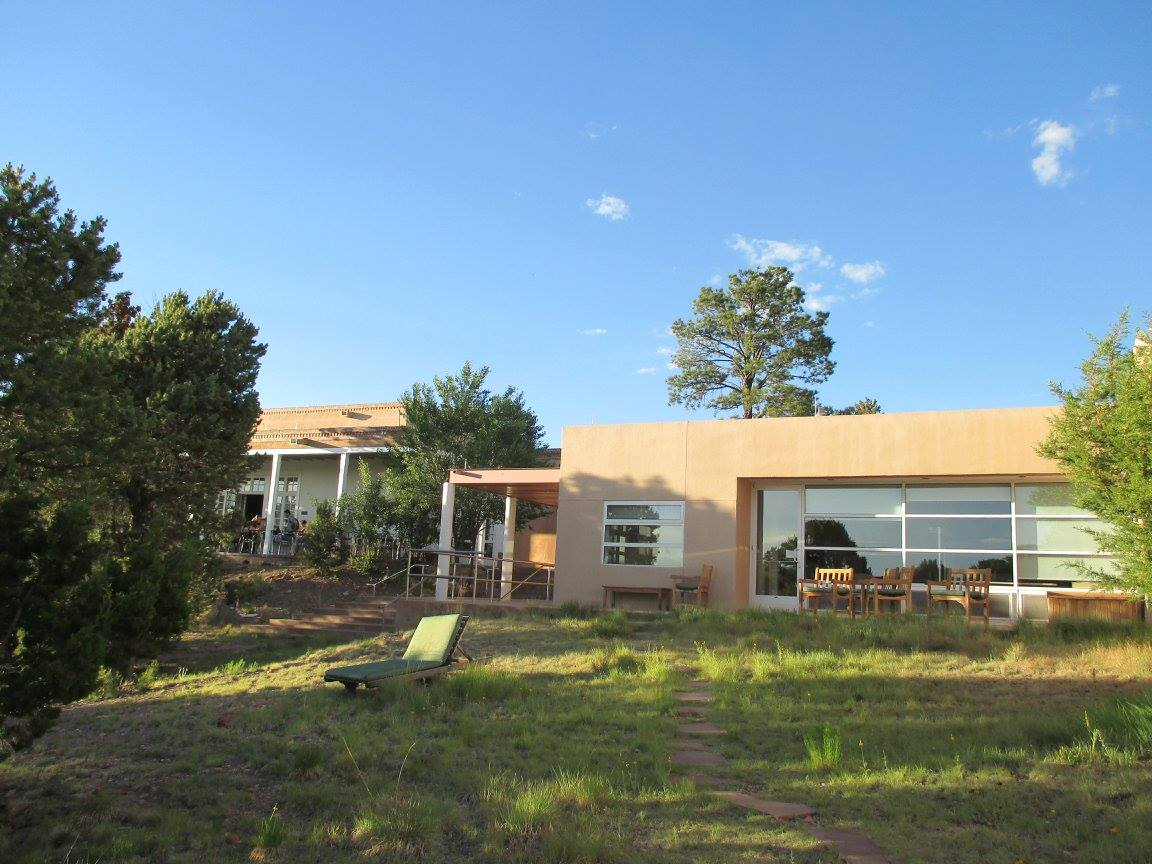
\includegraphics[width=\textwidth]{figures/pic_sfi}\\
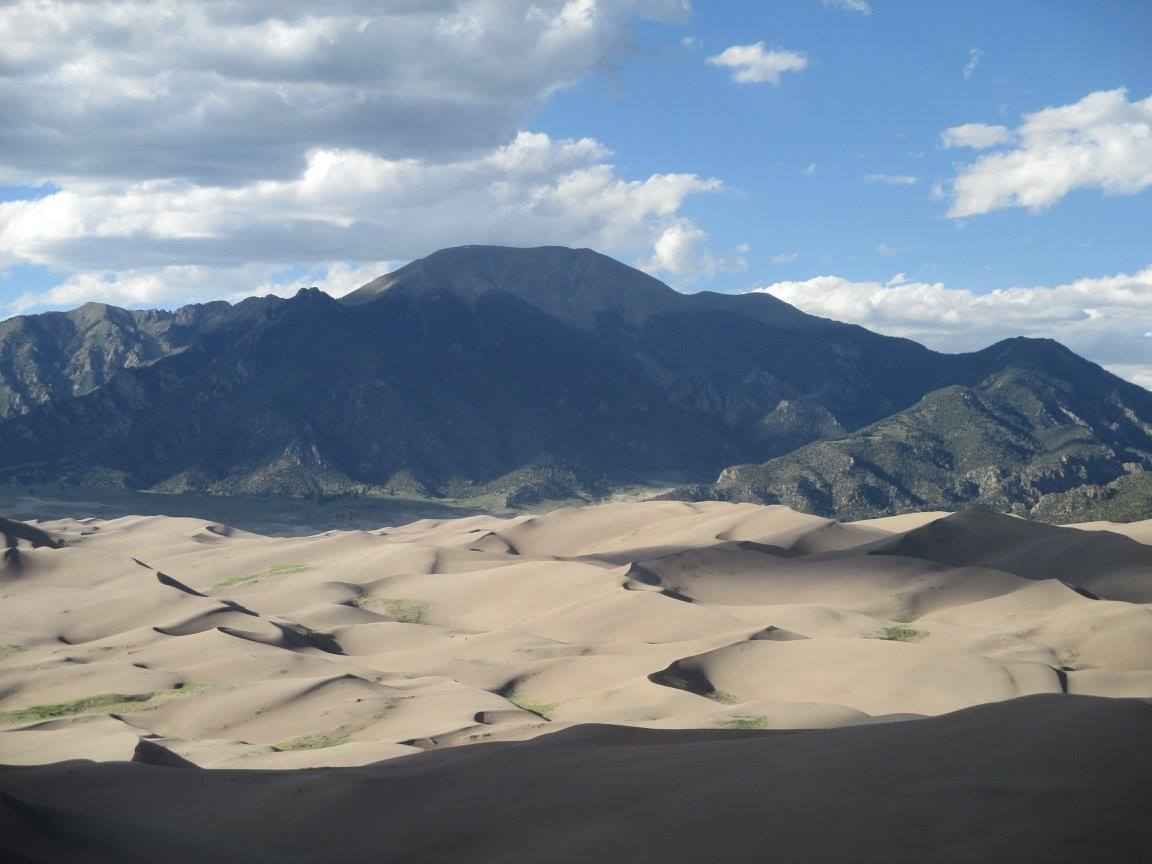
\includegraphics[width=\textwidth]{figures/pic_dunes}\\
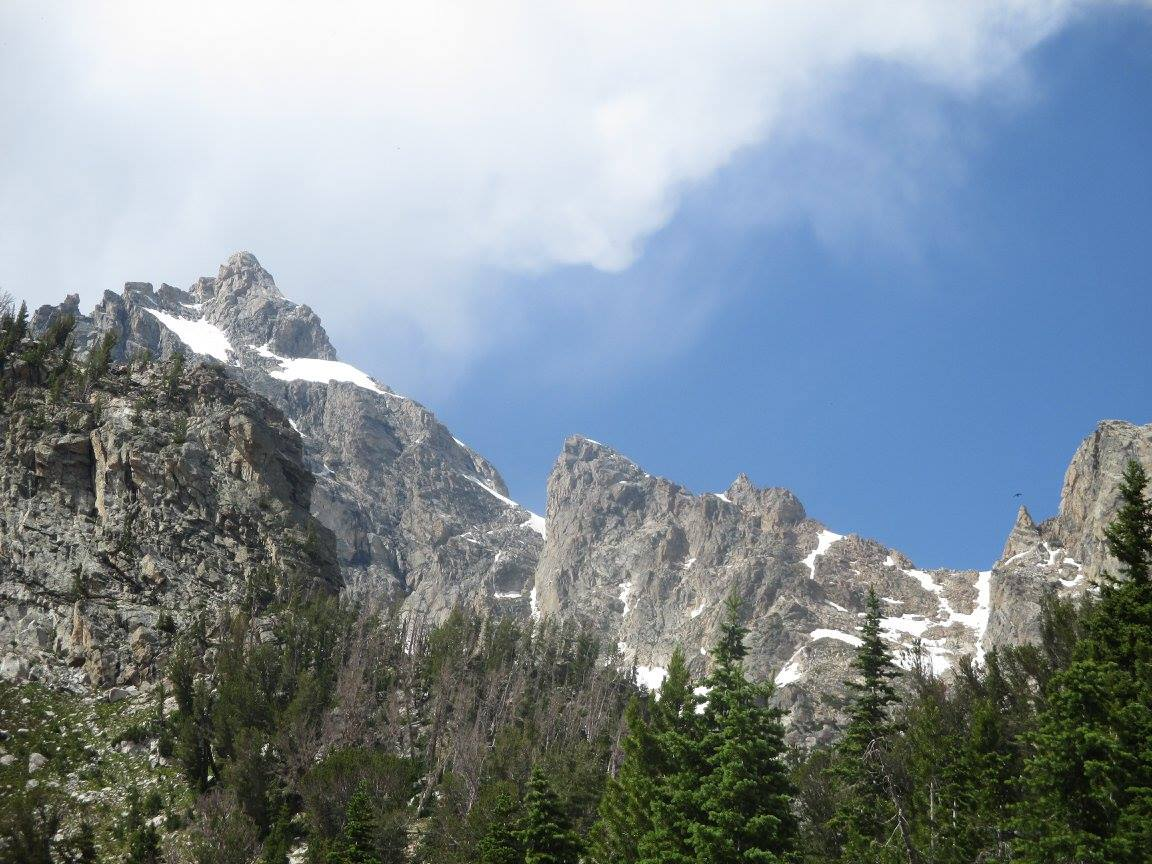
\includegraphics[width=\textwidth]{figures/pic_grdteton}
\end{column}
\begin{column}{0.5\textwidth}
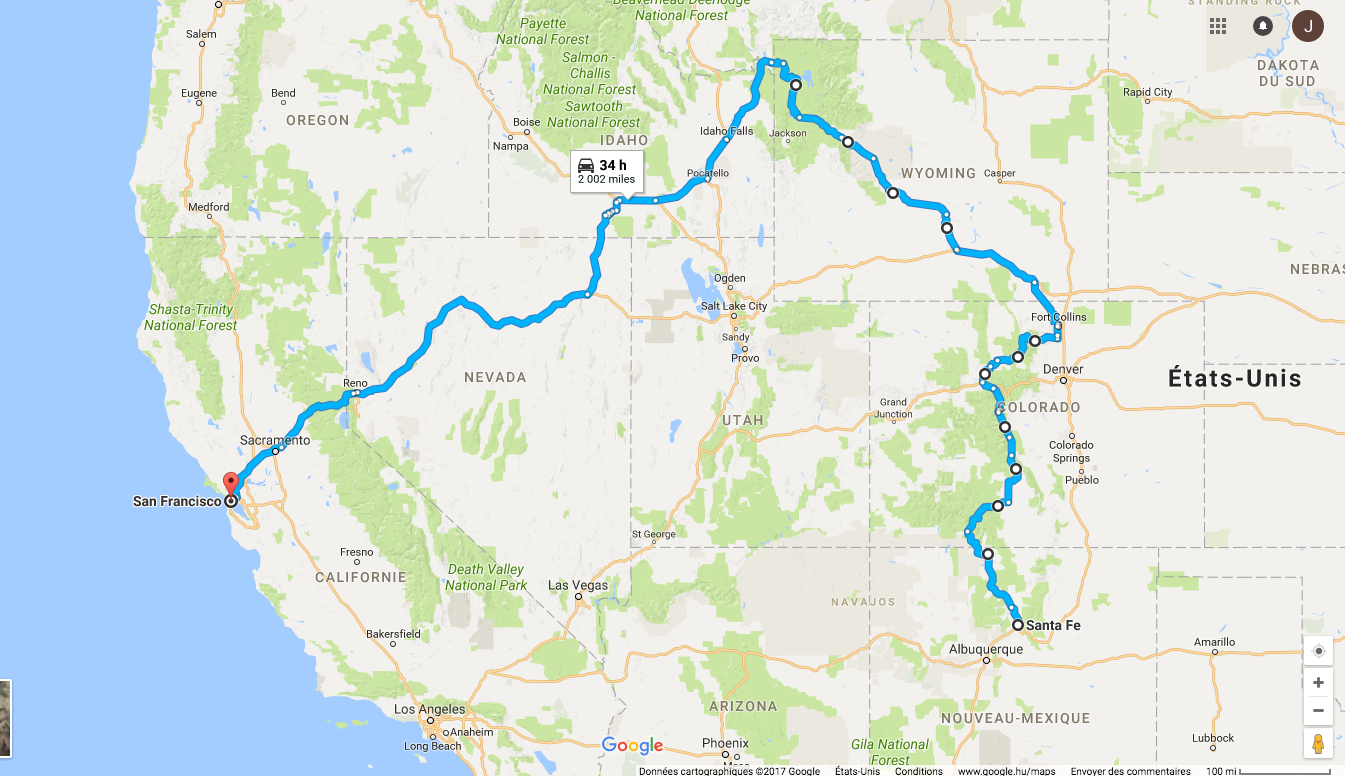
\includegraphics[width=\textwidth]{figures/roadtrip}
\end{column}
\begin{column}{0.25\textwidth}

\includegraphics[width=\textwidth]{figures/pic_rockies}\\
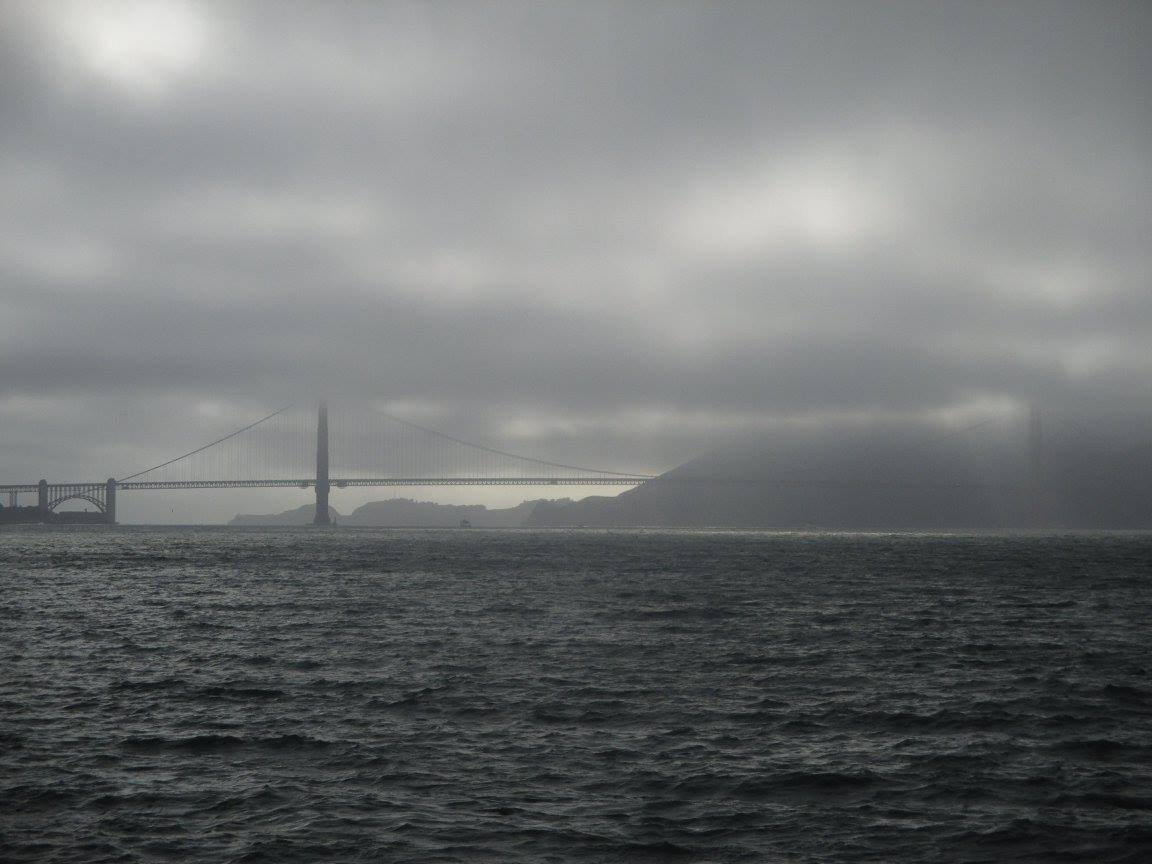
\includegraphics[width=\textwidth]{figures/pic_sf}\\
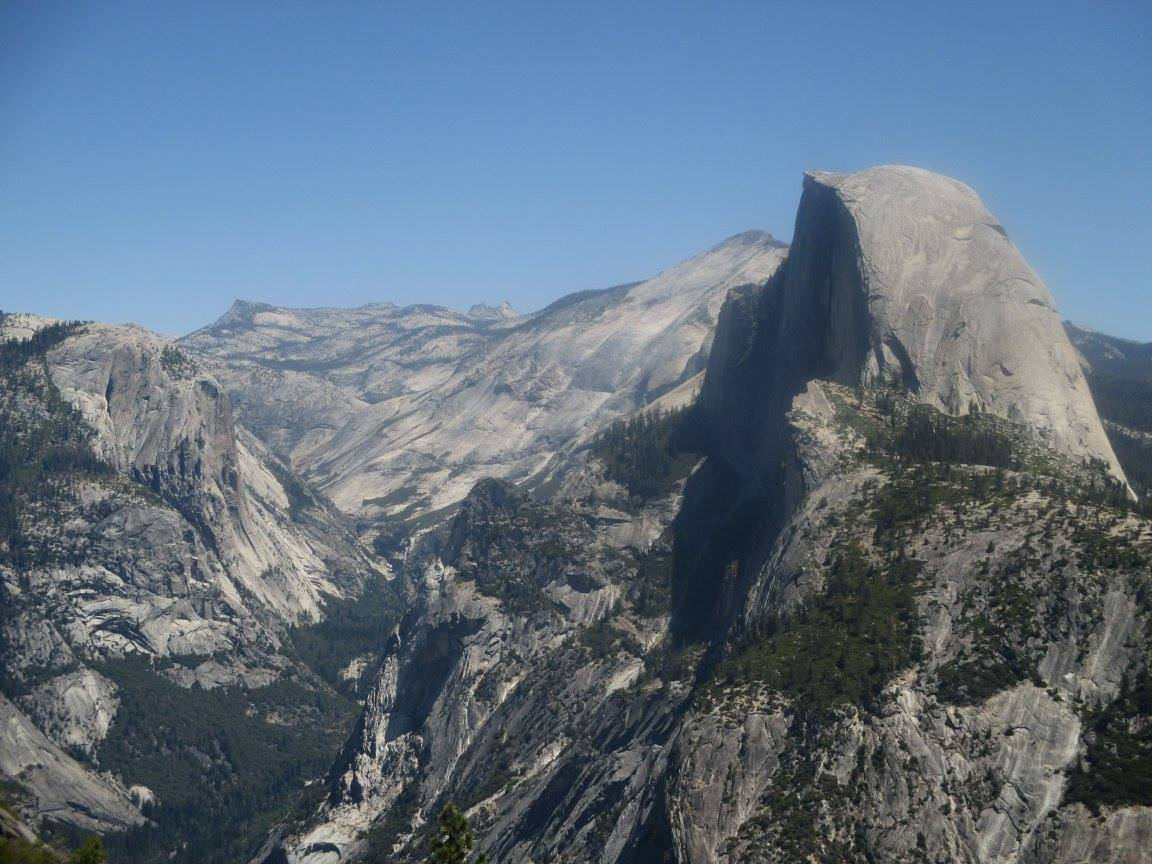
\includegraphics[width=\textwidth]{figures/pic_yosemite}
\end{column}
\end{columns}

}


\sframe{Geography and Fuel prices}{

$\rightarrow$ In the US you fuel your (necessary big) car everywhere and everyday, and directly feel the strong variability of prices !

\justify

\textit{Spatio-temporal variability of Fuel Price captures geographical properties of a particular energy market, of the transportation system, of interactions between transportation and territories.}

\bigskip

\textbf{Diverse approaches mostly by economists :}

\begin{itemize}
\item \cite{rietveld2001spatial} cross-border variability
\item \cite{gregg2009temporal} influence on carbon emissions
\item \cite{combes2005transport} effective transportation costs
\item \cite{gautier2015dynamics} from crude oil price to retail price
\end{itemize}



}



\sframe{Exploratory Spatial analysis}{

\justify

\textbf{Research Objective : } \textit{Construction and Exploratory analysis of a large and detailed dataset of US fuel retail price, focusing on spatio-temporal variability}

\bigskip
\bigskip

$\rightarrow$ Focus on geographical patterns and structures

\medskip

$\rightarrow$ Complementarity of spatial analysis methods

\medskip

$\rightarrow$ Interdisciplinary point of view on a fundamentally heterogenous system

}


%%%%%%%%%%%%%%%%%
\section{Methods and Results}
%%%%%%%%%%%%%%%%%



\sframe{Dataset Construction}{

\justify

\textit{Crowdsourced Big Data as a new way to unveil structure of complex socio-technical systems}

\bigskip


$\rightarrow$ Construction of a large scale dataset covering most of US fuel stations on two month

\bigskip

\textbf{Requirements : } Flexibility, performance and anonymity

\medskip

\textbf{Architecture : } Pool of proxy tasks to pipe requests through \texttt{tor}; manager monitors and launches collection tasks; subtasks crawl and parse target webpages.

\medskip

\textit{Dataset available upon request, ``grey area'' of semi-open data.}

\medskip


}



\sframe{Dataset Summary}{

\begin{itemize}
\item $41\cdot 10^6$ unique observations, between January and March 2017\\$\rightarrow$ 5,204,398 gas station - day observations for main purchase mode and regular fuel, used in the analysis, aggregated at the county level
\item Socio-economic data from US Census Bureau
\end{itemize}


\bigskip

\begin{table}
\centering
\caption{Descriptive statistics on Fuel Price (\$ per gallon)}
\begin{tabular}{ccccccc}
\textbf{Mean} & \textbf{Std. Dev.} & \textbf{p10} & \textbf{p25} & \textbf{p50} & \textbf{p75} & \textbf{p90} \\
\hline
\cr
2.28 & 0.27 &  2.02  &  2.09  &  2.21  &  2.39  &  2.65  \\
\hline
\end{tabular}
\end{table}

}




\sframe{Data Exploration}{

\textit{Interactive web-application for spatio-temporal exploration}

\bigskip

\centering

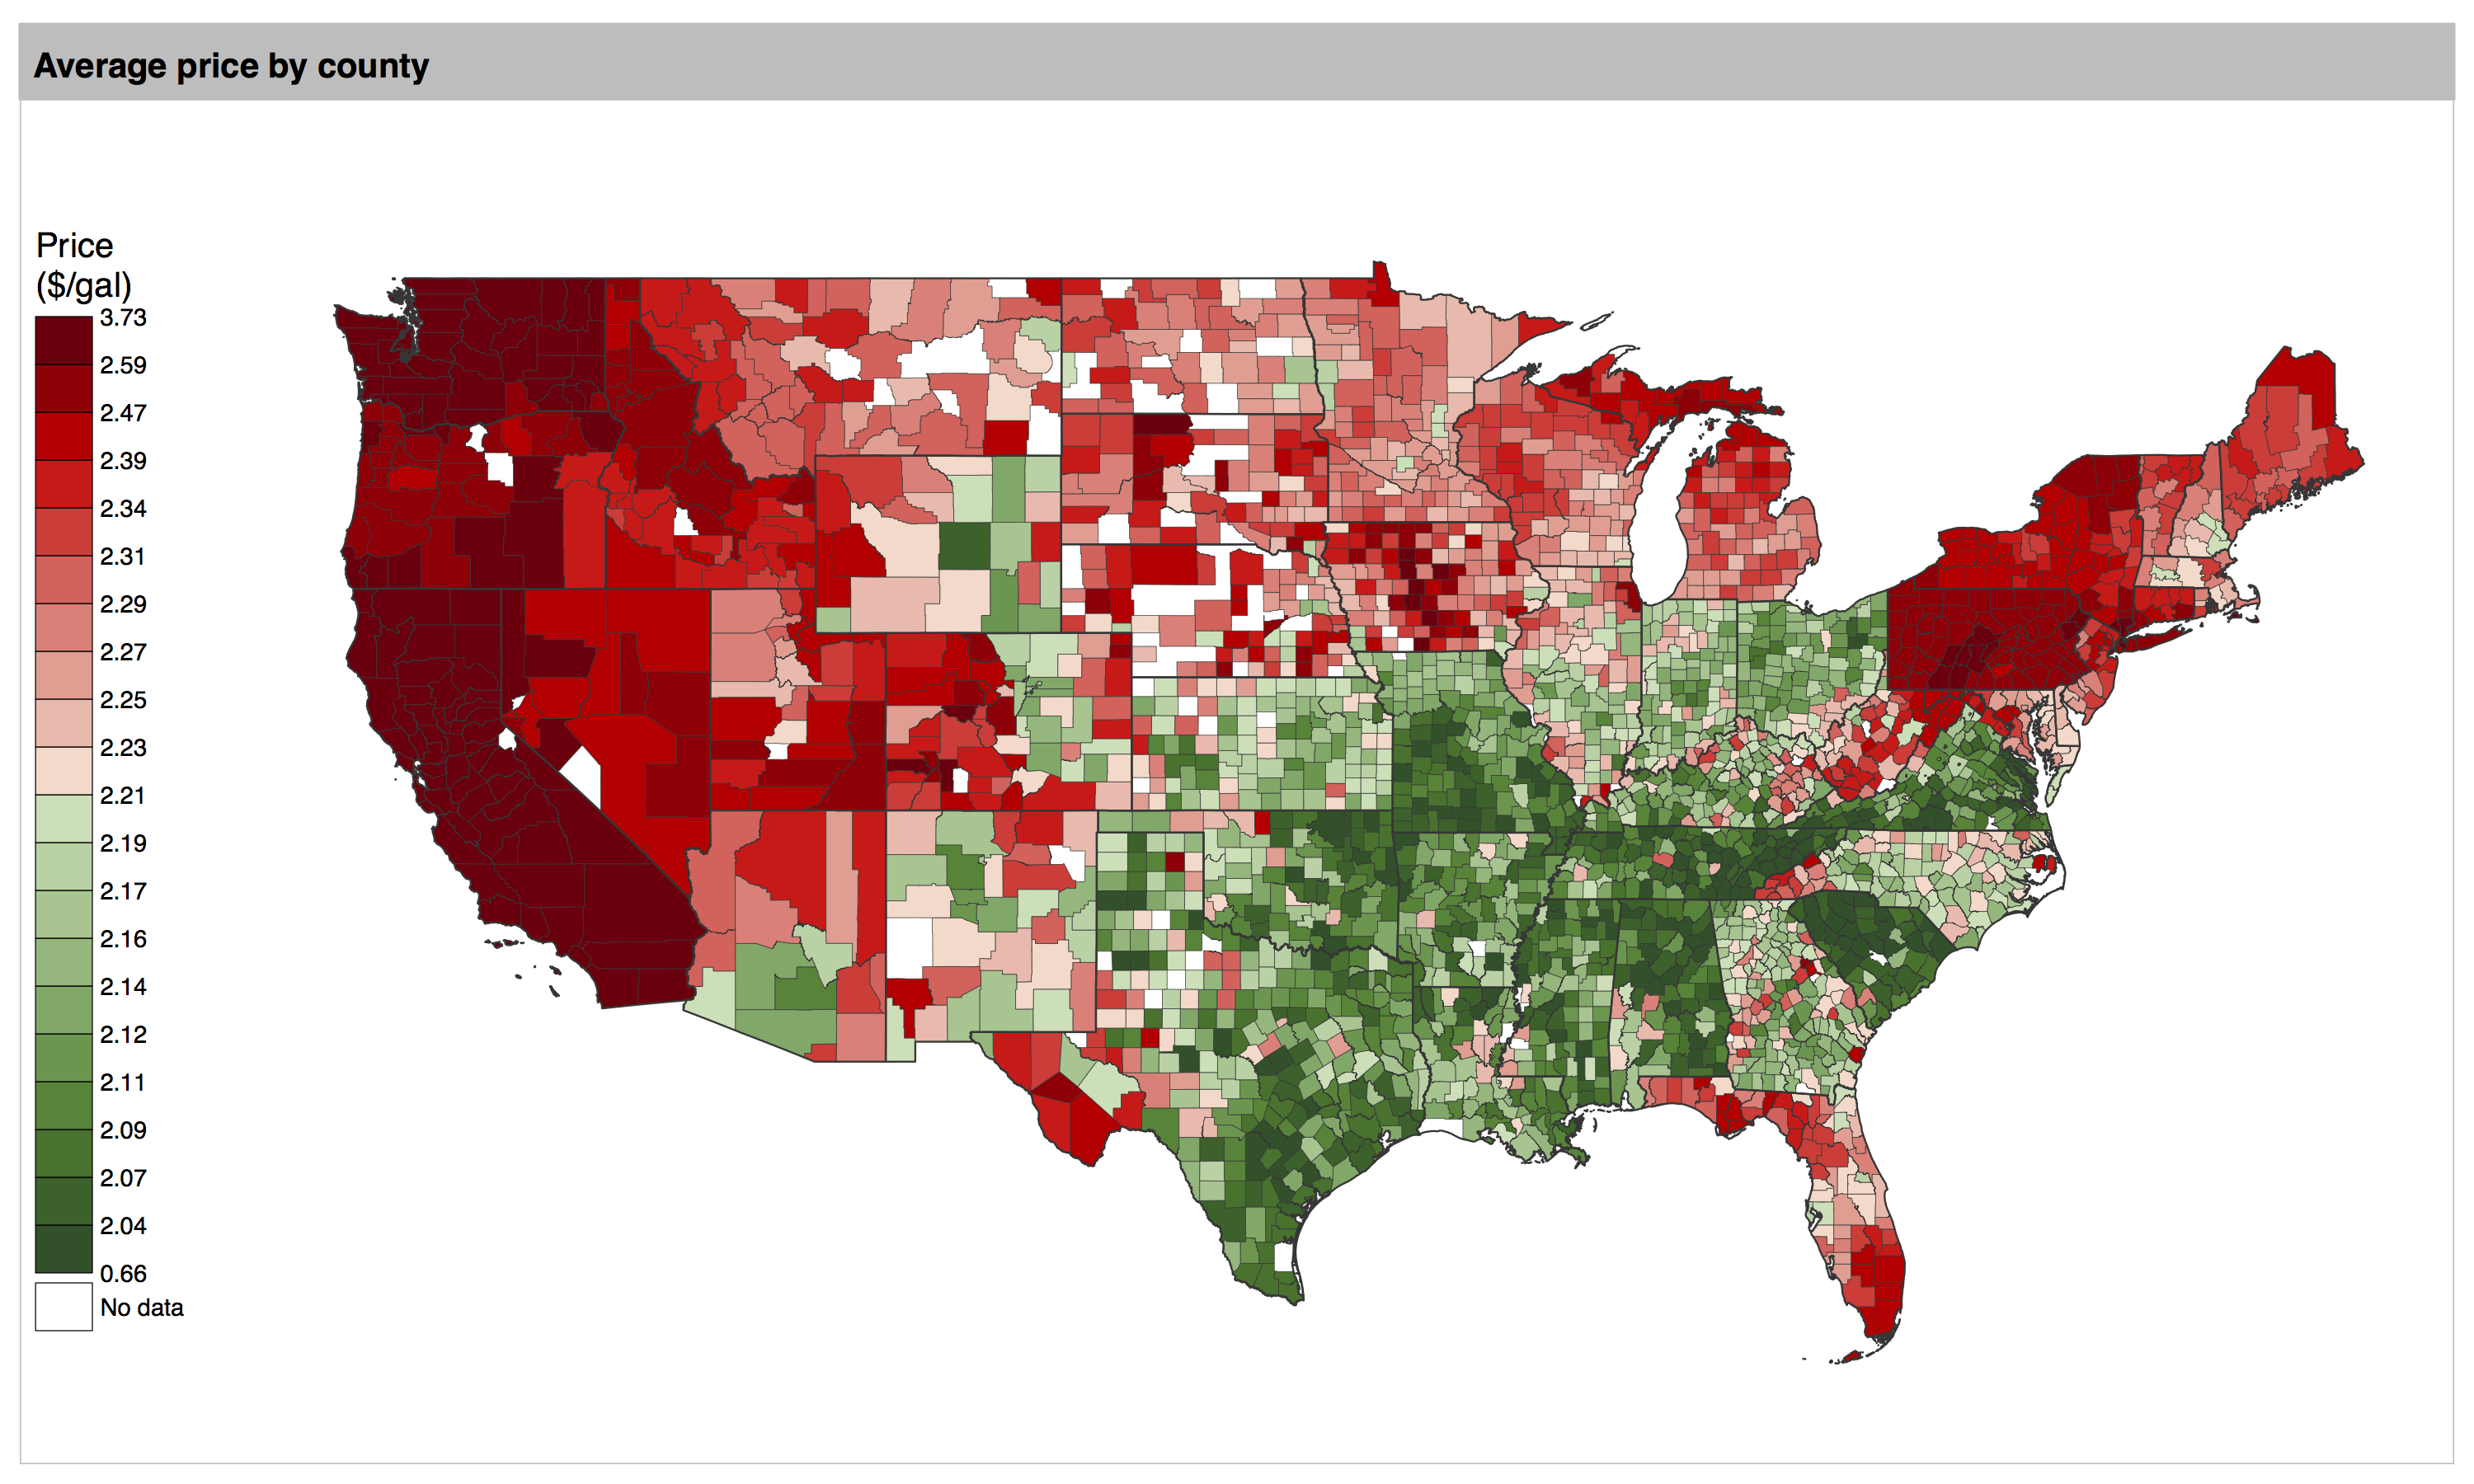
\includegraphics[width=\textwidth]{figures/average_regular_map}

%\textit{Average prices in time by county for regular fuel}

}




\sframe{Spatio-temporal correlations}{

\textit{Variability in space and time of Moran spatial auto-correlation index unveils strong non-stationnarity}

\bigskip

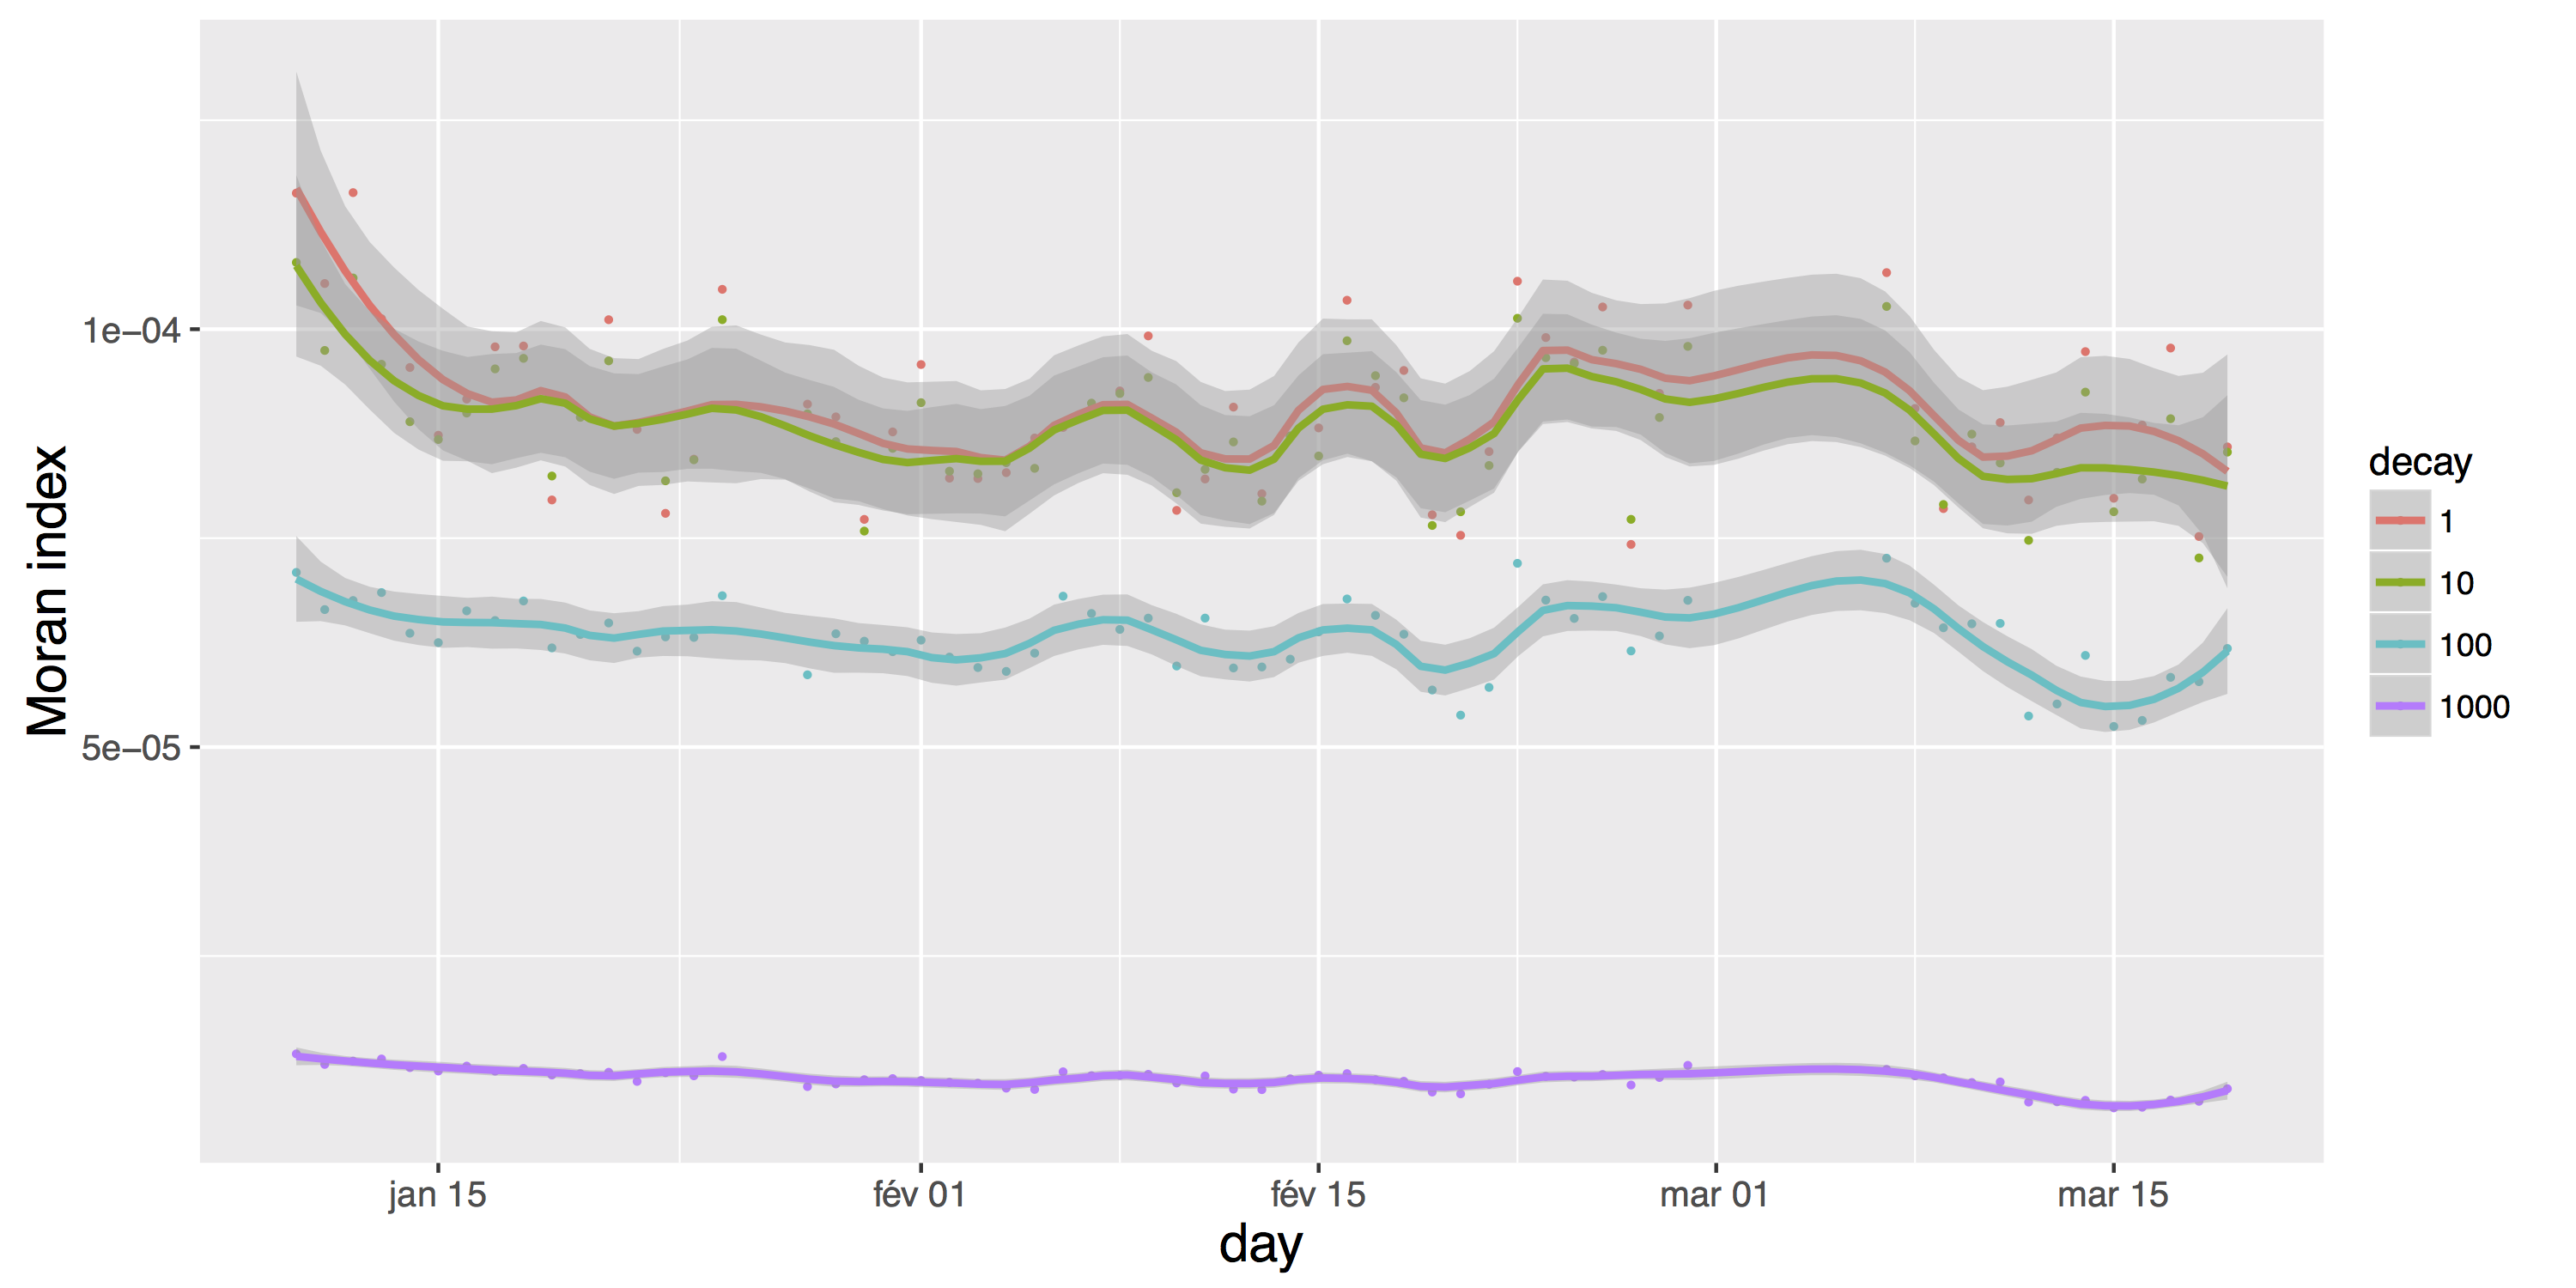
\includegraphics[width=0.5\textwidth,height=0.6\textheight]{figures/moran_days}
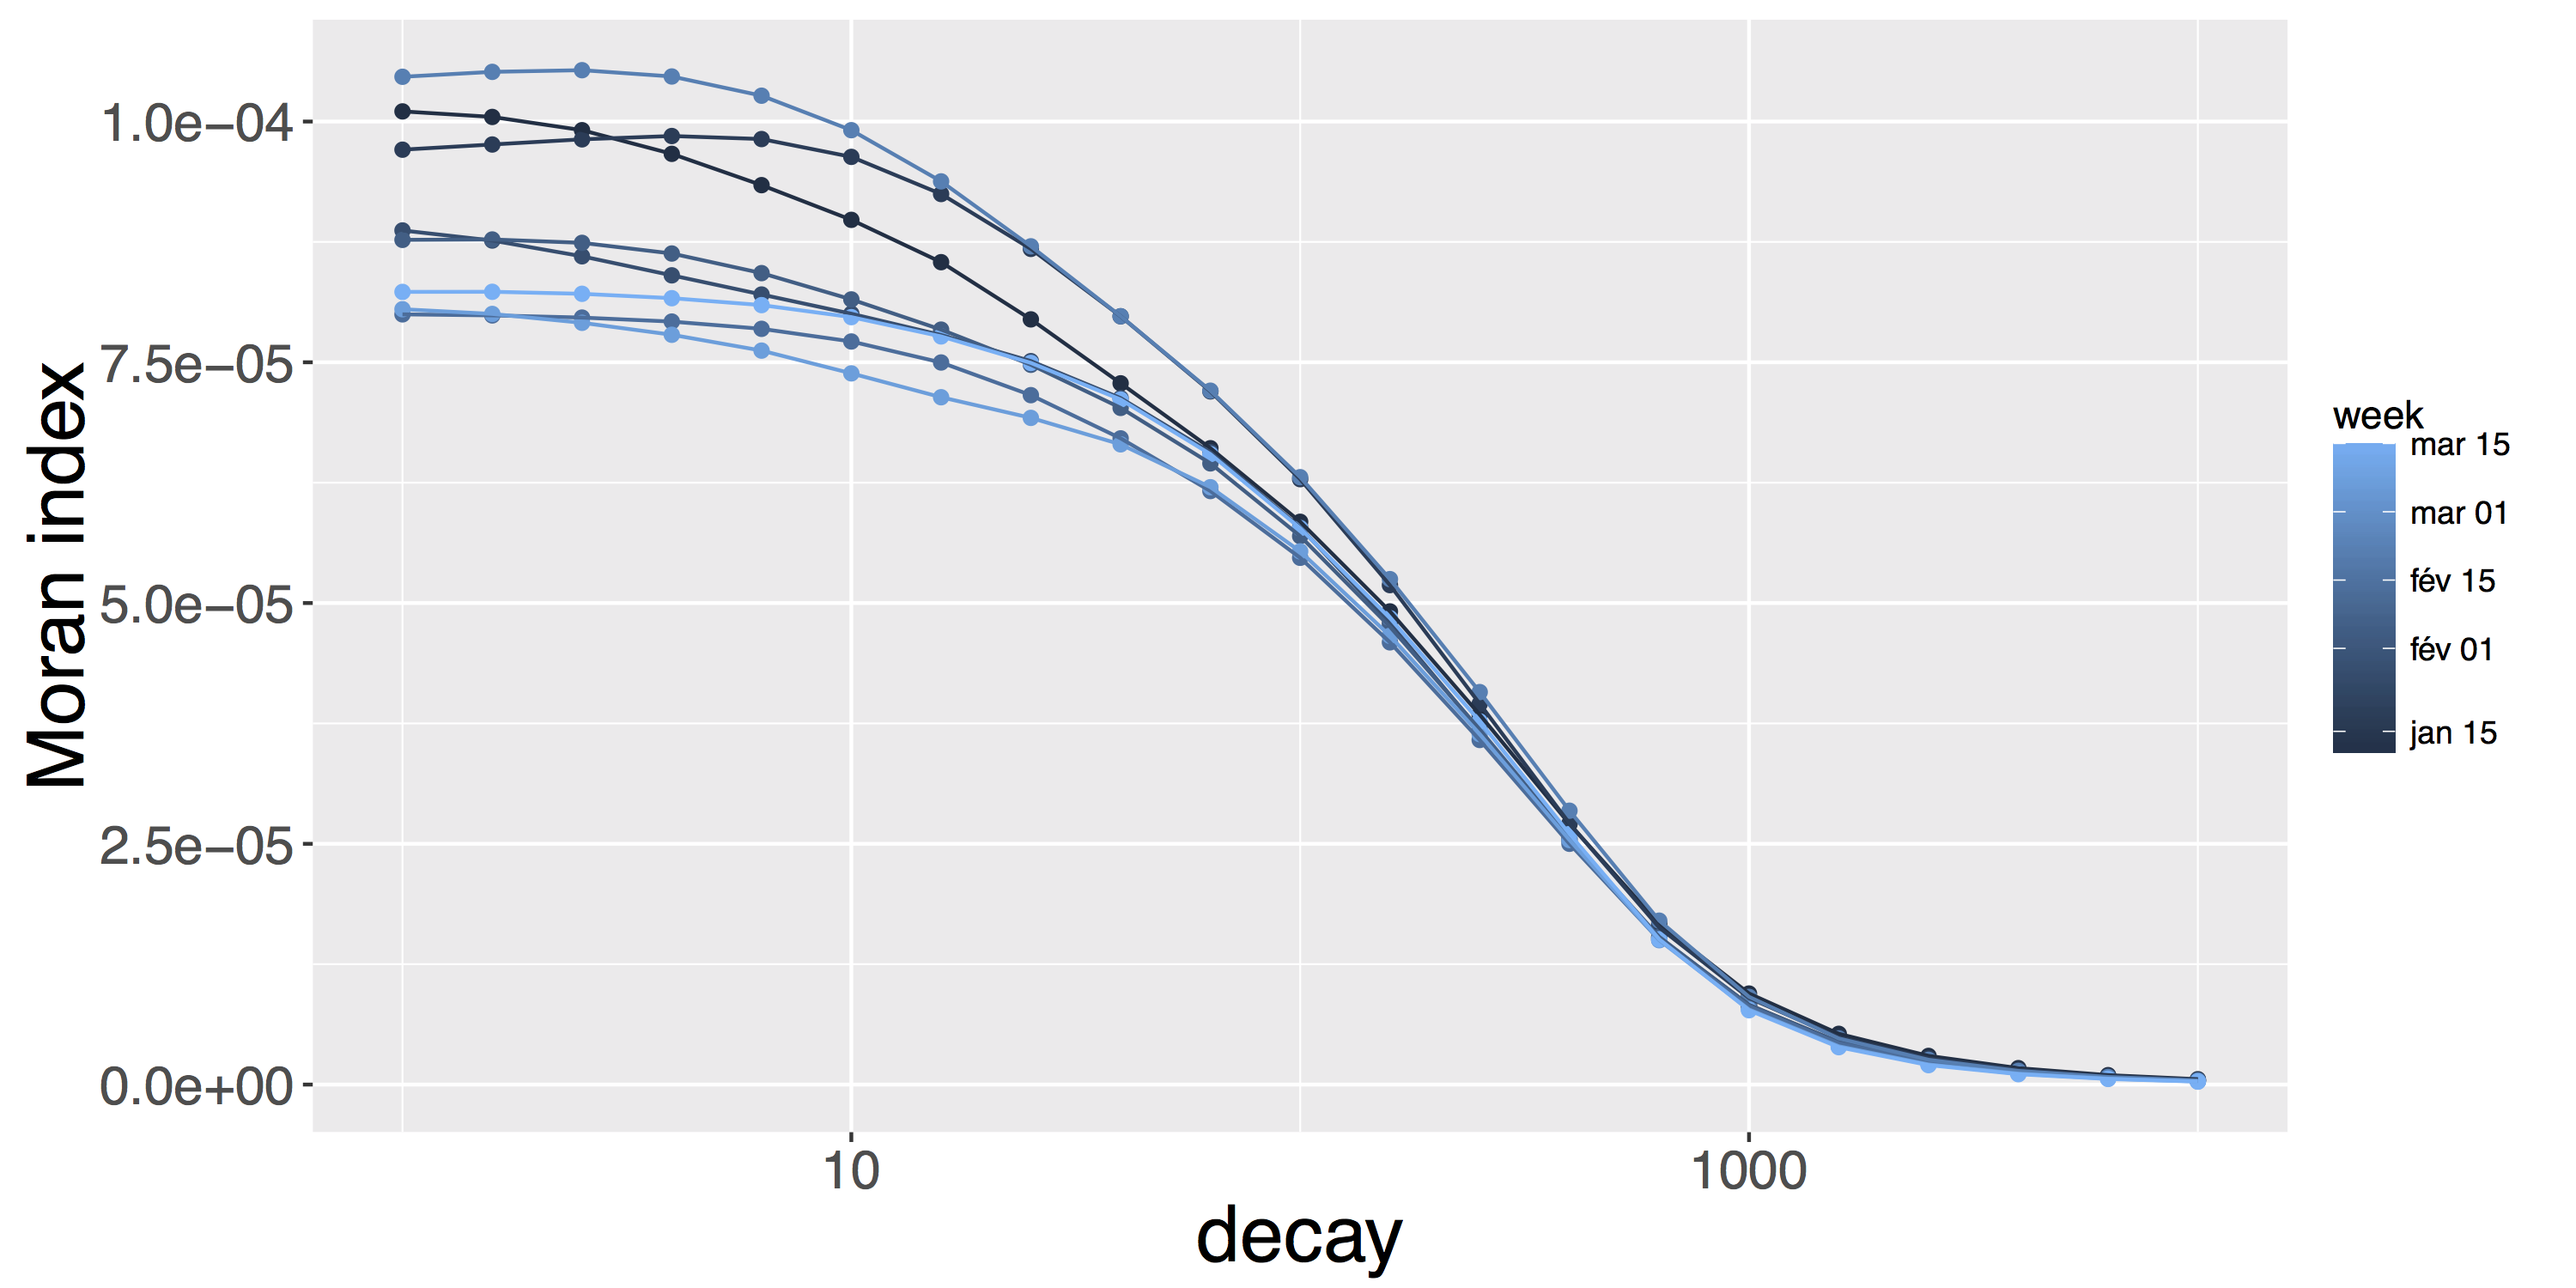
\includegraphics[width=0.5\textwidth,height=0.6\textheight]{figures/moran_decay_weeks}

}


\sframe{Geographically Weighted Regression}{


\begin{itemize}
\item Geographically Weighted Regression (GWR)~\cite{brunsdon1996geographically} to tackle spatial non-stationarity : capturing a variable influence in space of explicative variables for prices
\item Multi-modeling using corrected AIC for model selection : find the best model and the best bandwidth controlling for overfitting
\end{itemize}

\bigskip
\bigskip

\textbf{Best model :}  $price = \beta\cdot\left( income, wage, percapjobs\right)$ with an optimal bandwidth around 75km (22 neighbors with adaptive bandwidth), interpreted as spatial stationarity scale of price processes in relation to economic agents.

}


\sframe{Geographically Weighted Regression : Results}{

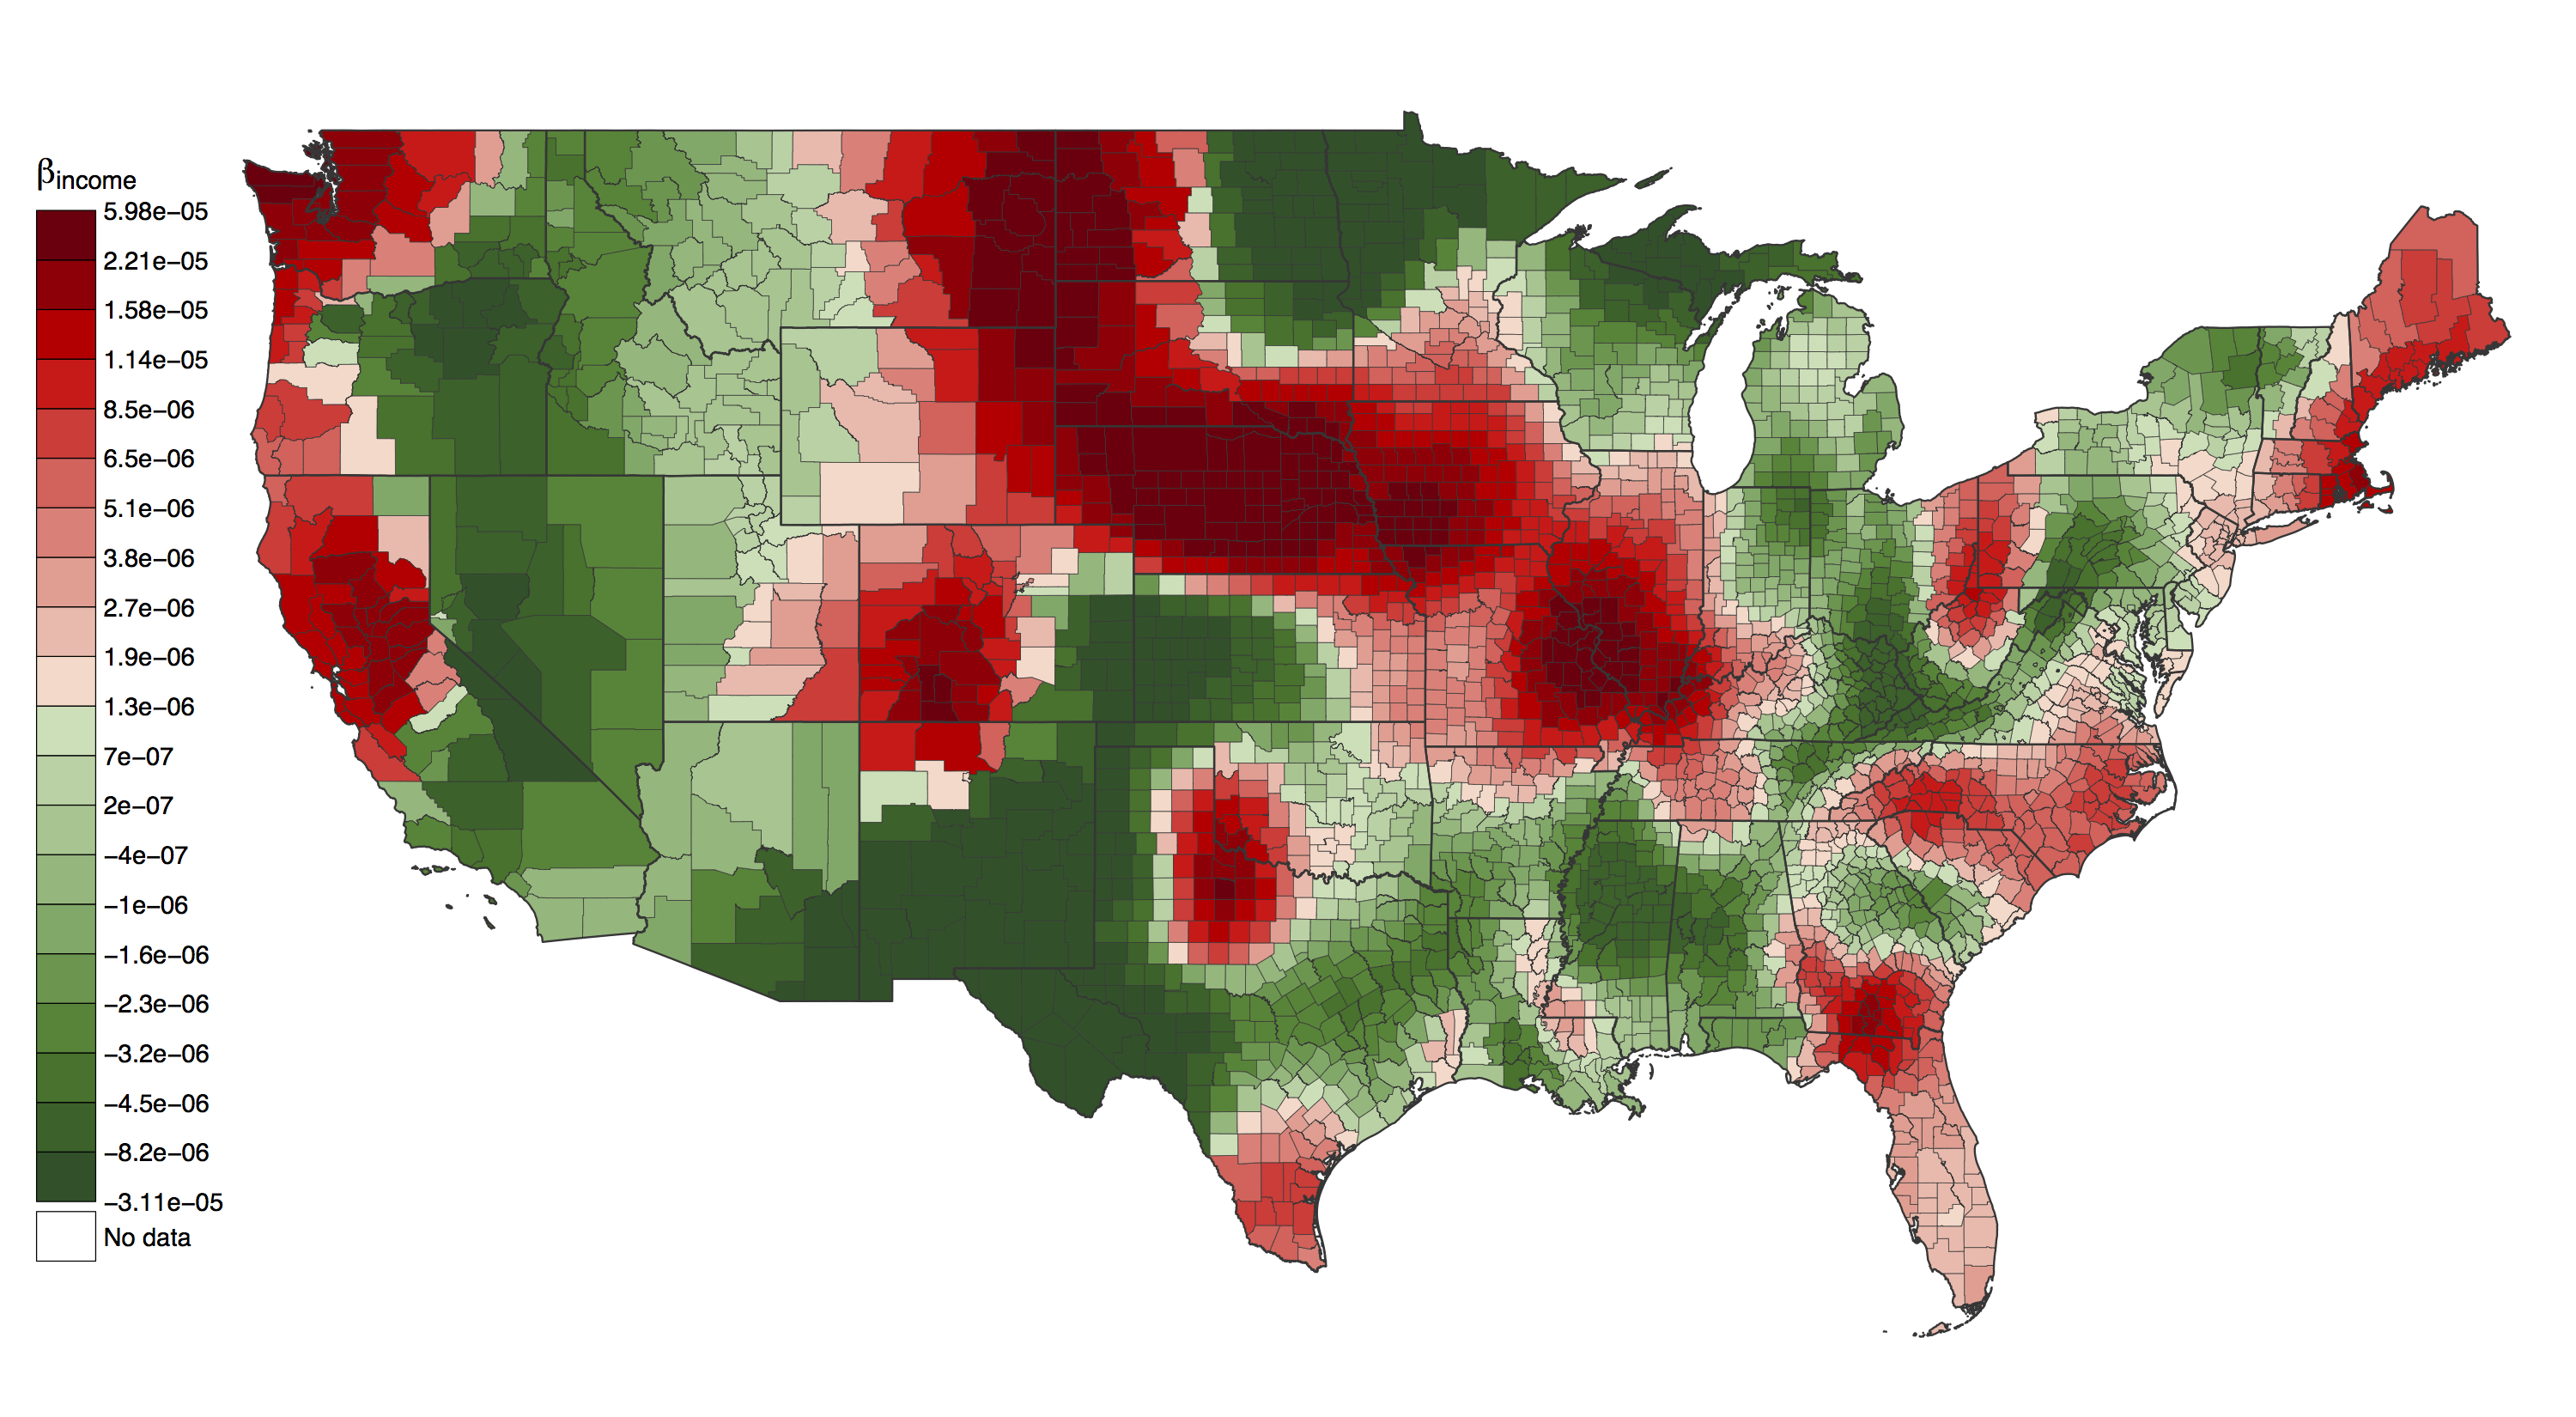
\includegraphics[width=0.5\textwidth,height=0.4\textheight]{figures/gwr_allbest_betaincome}
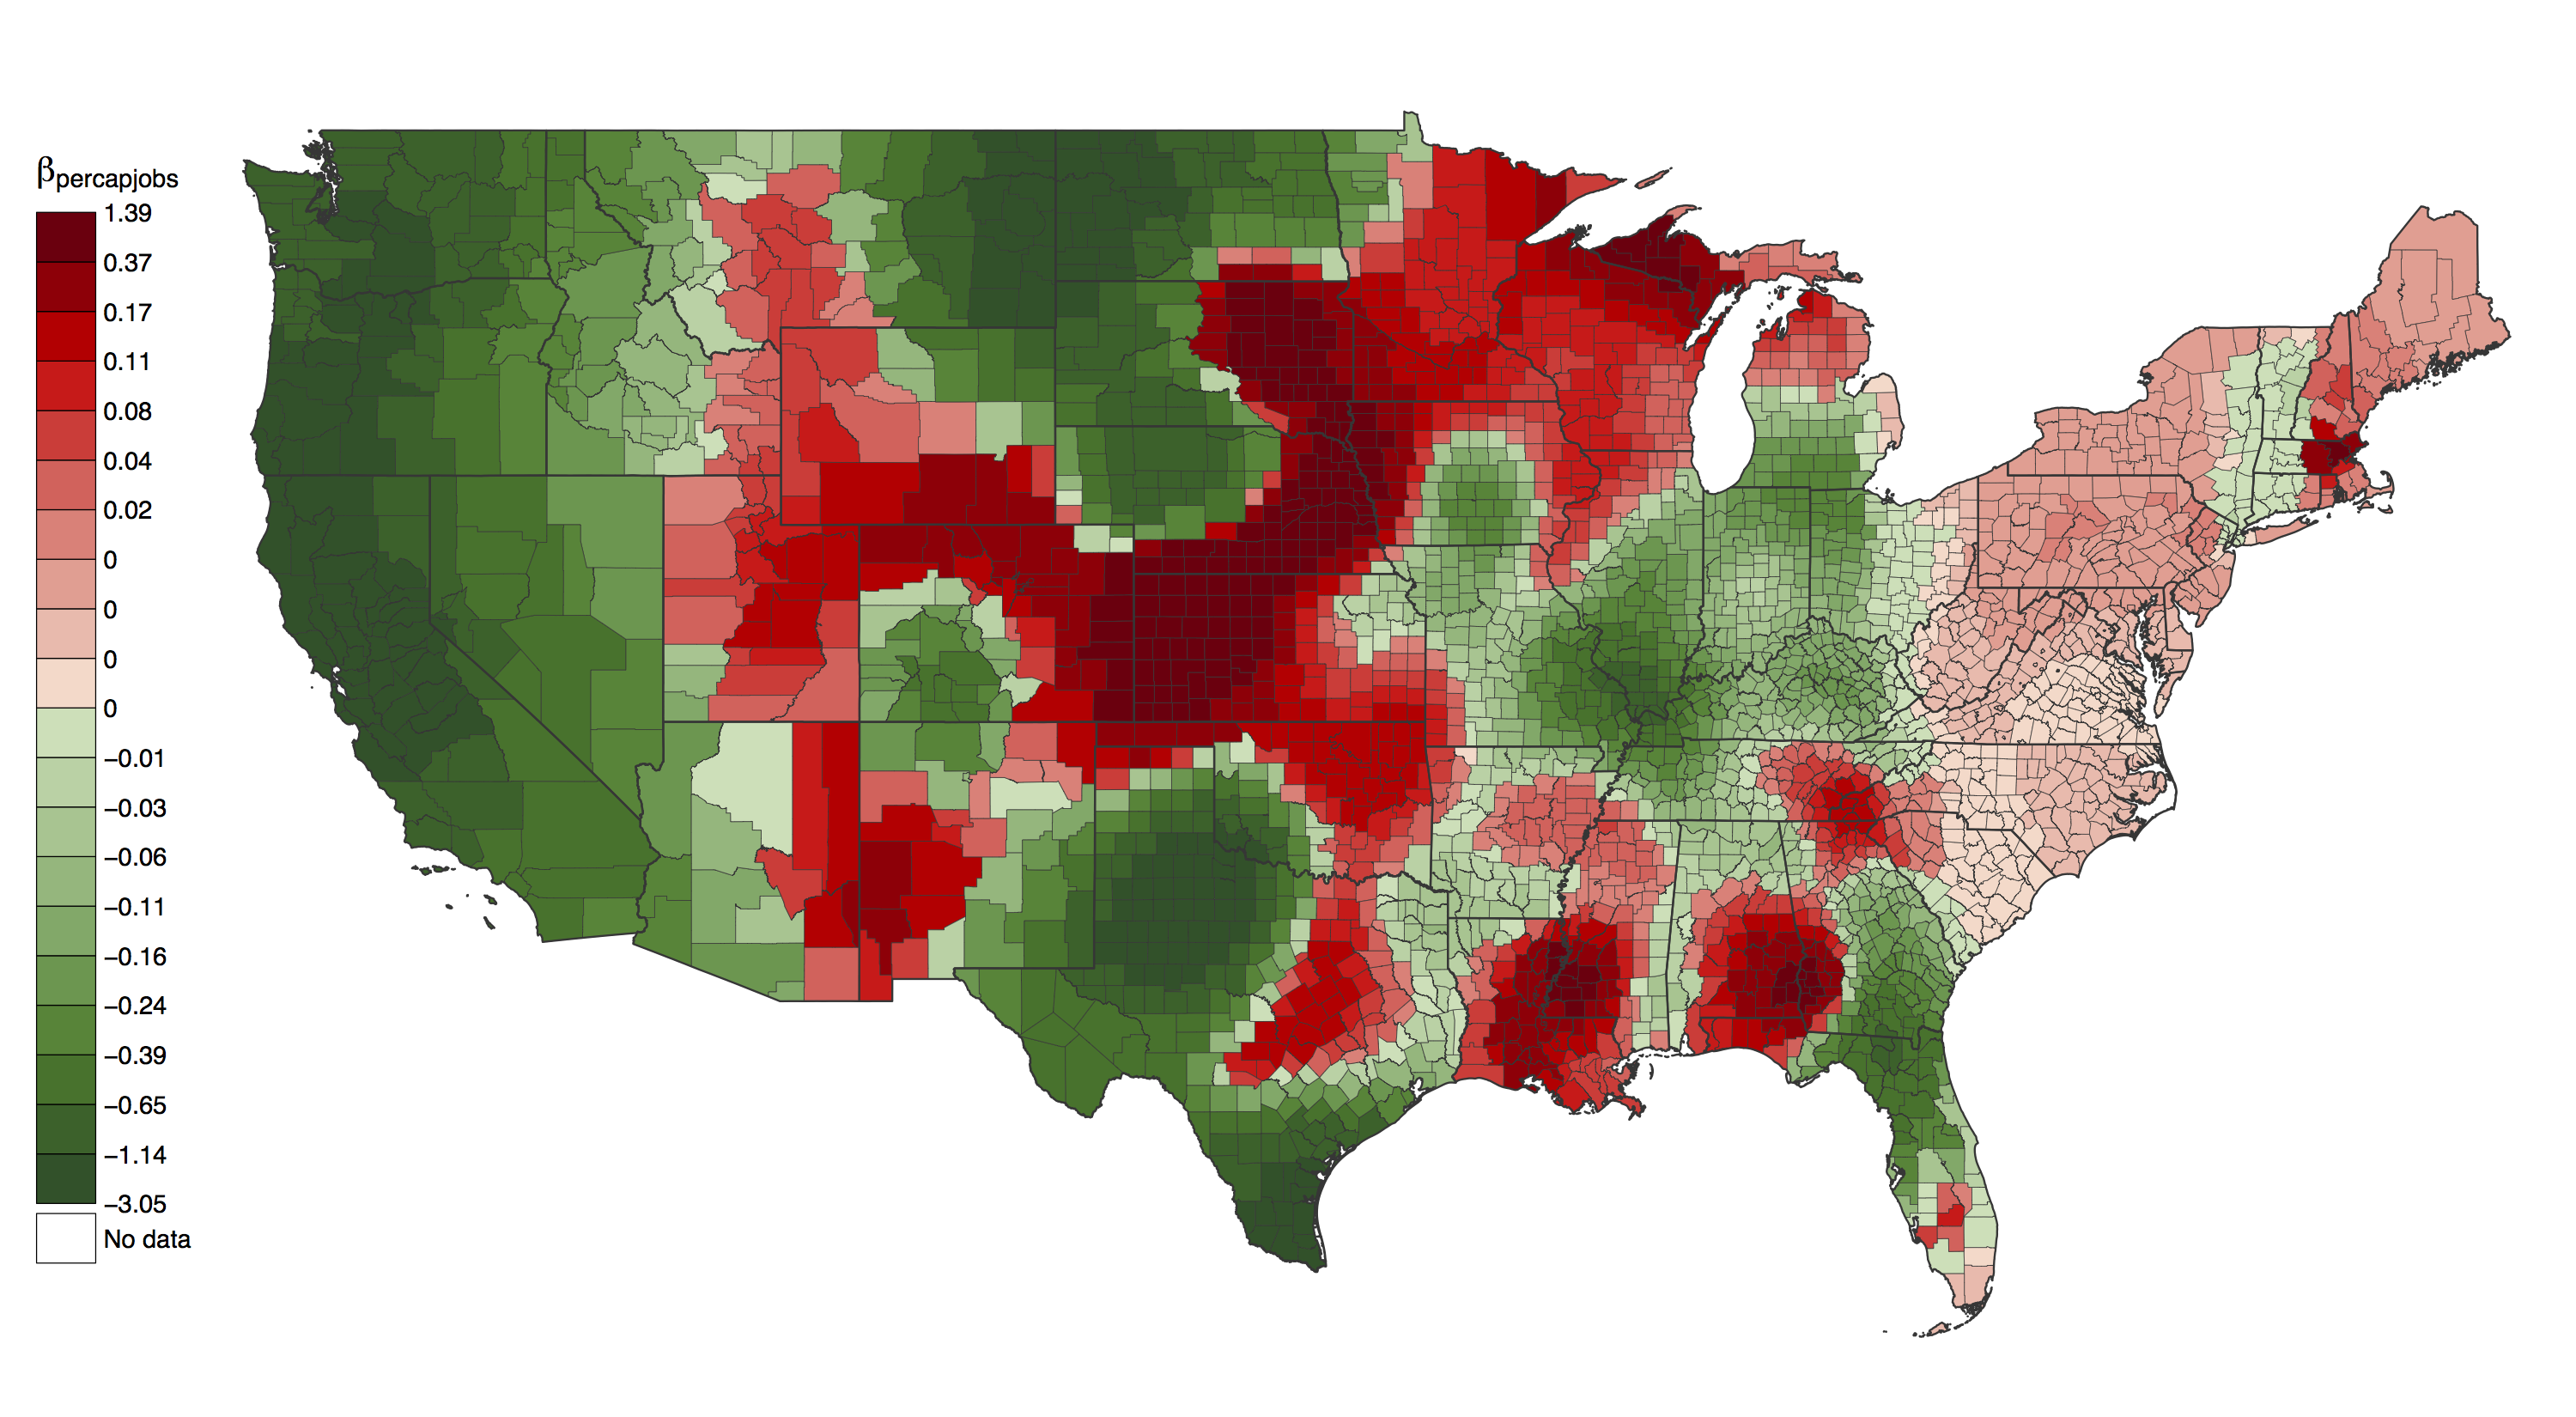
\includegraphics[width=0.5\textwidth,height=0.4\textheight]{figures/gwr_allbest_betapercapjobs}\\
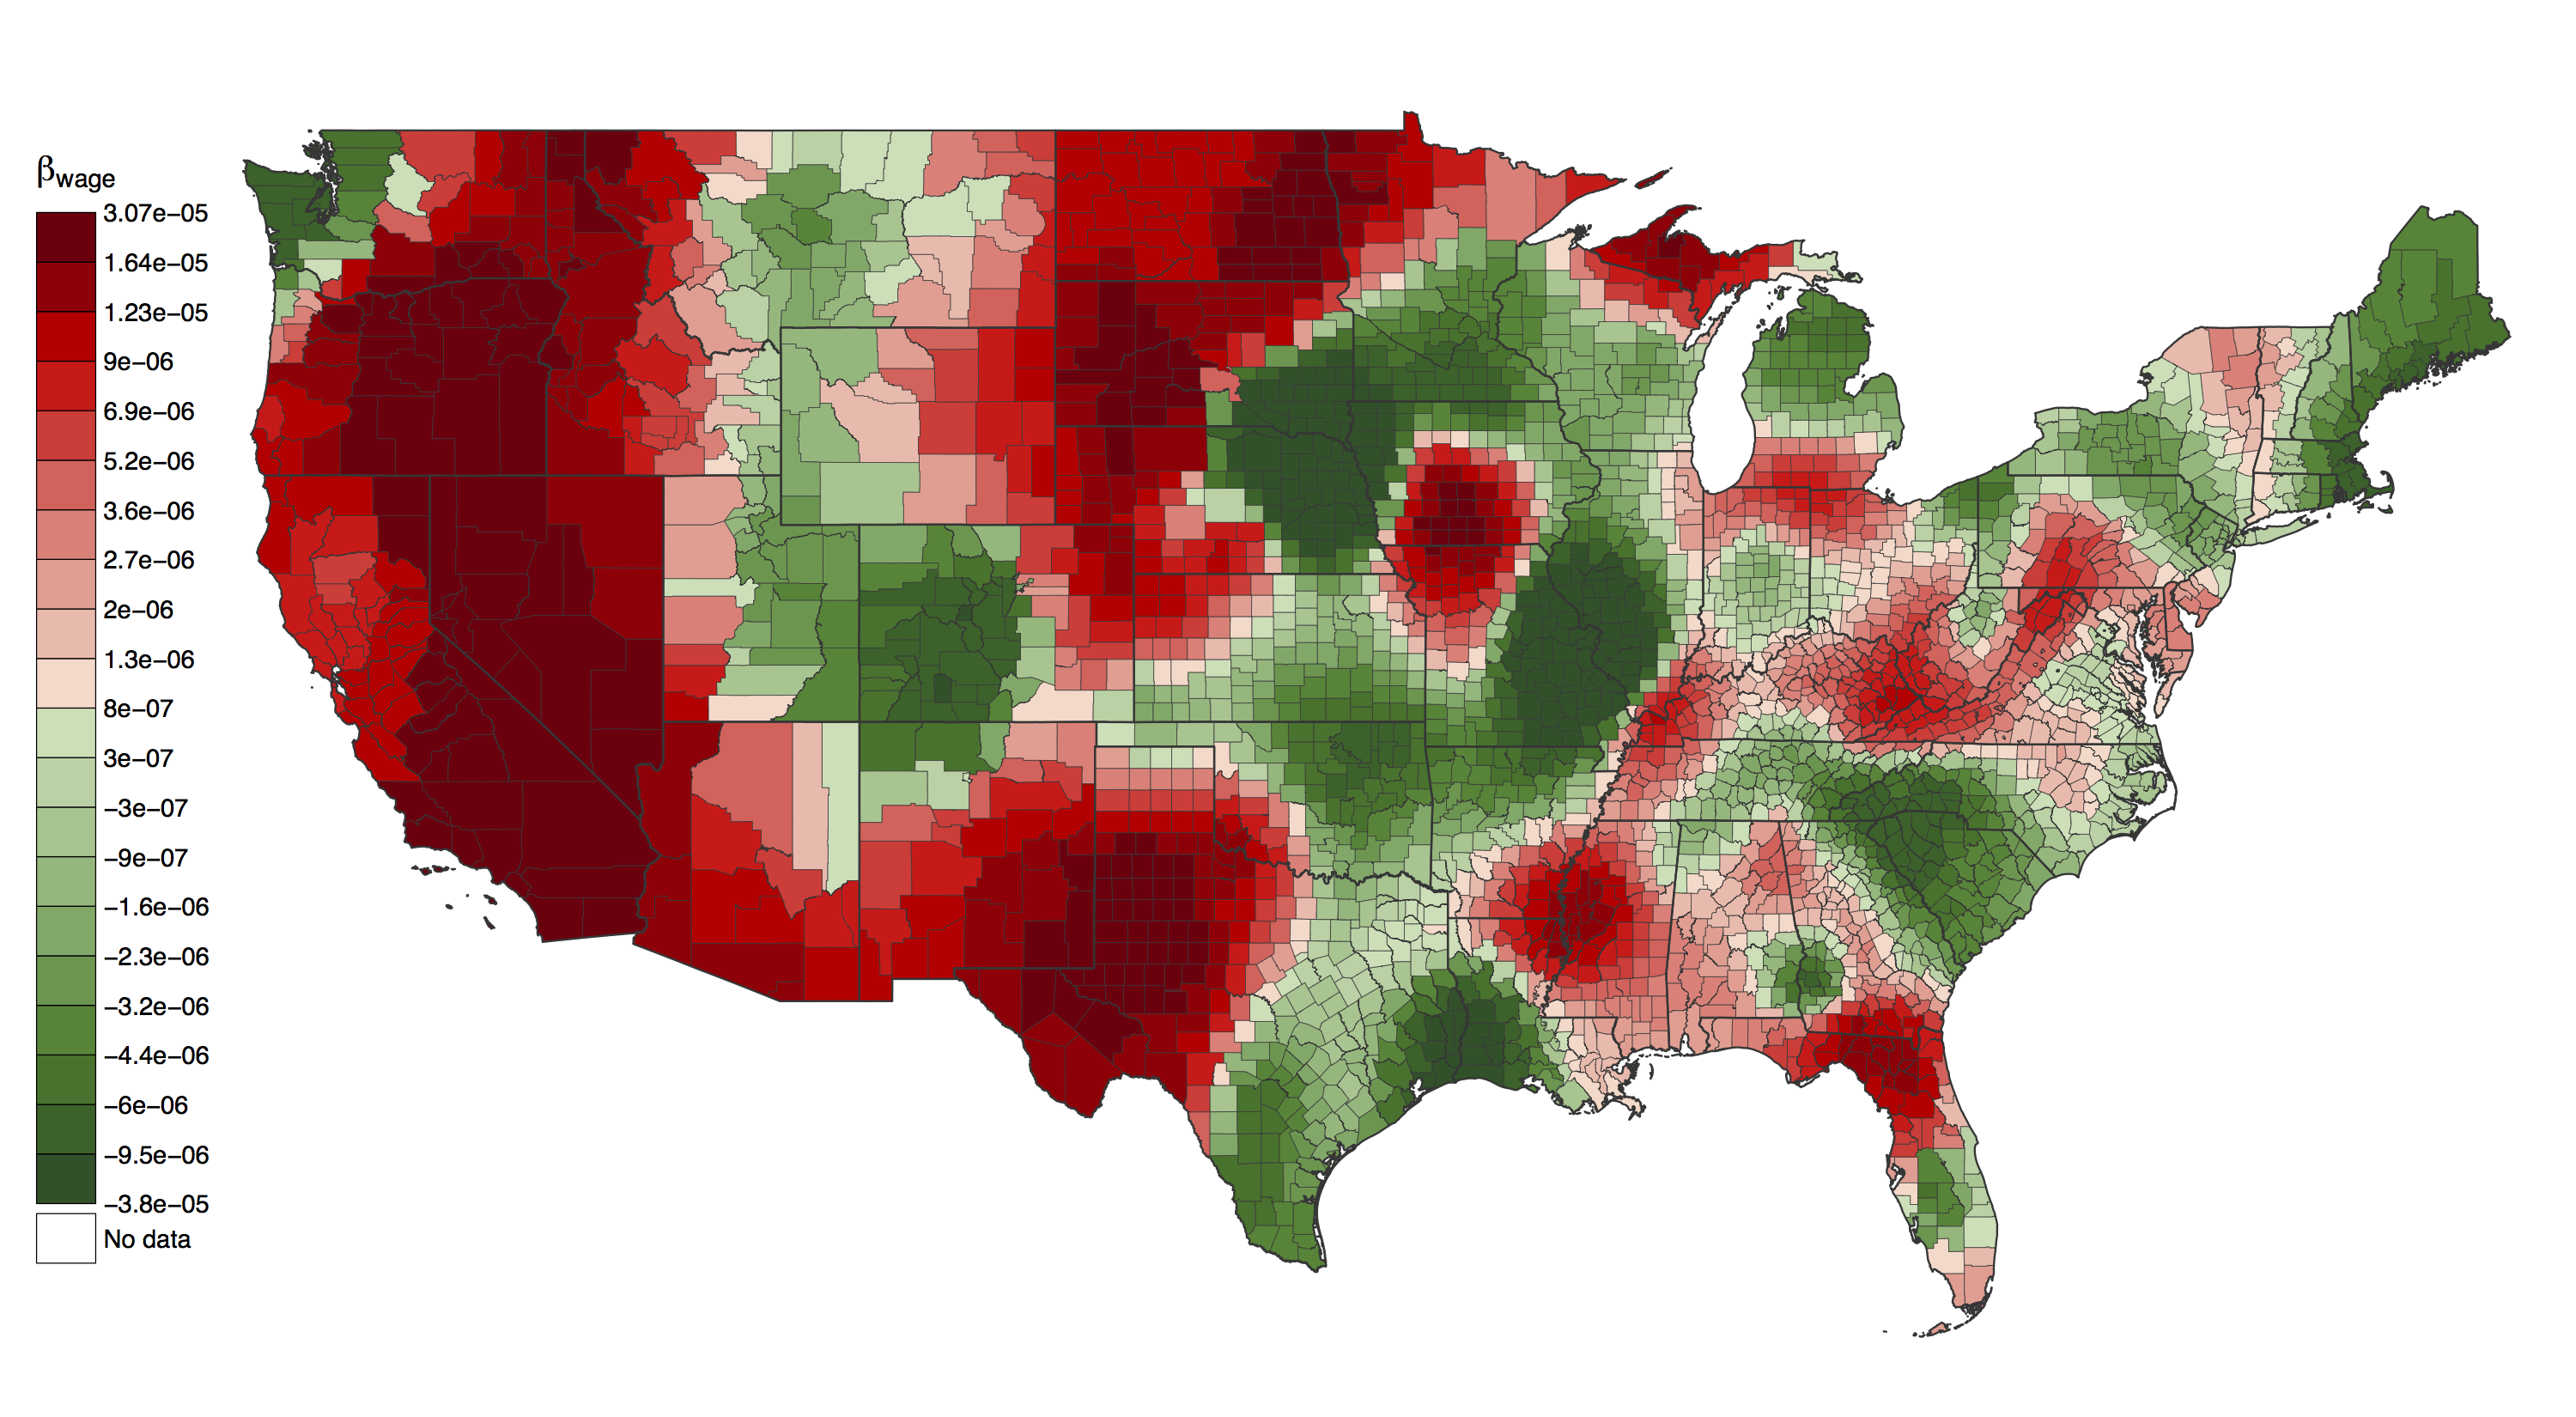
\includegraphics[width=0.5\textwidth,height=0.4\textheight]{figures/gwr_allbest_wage}
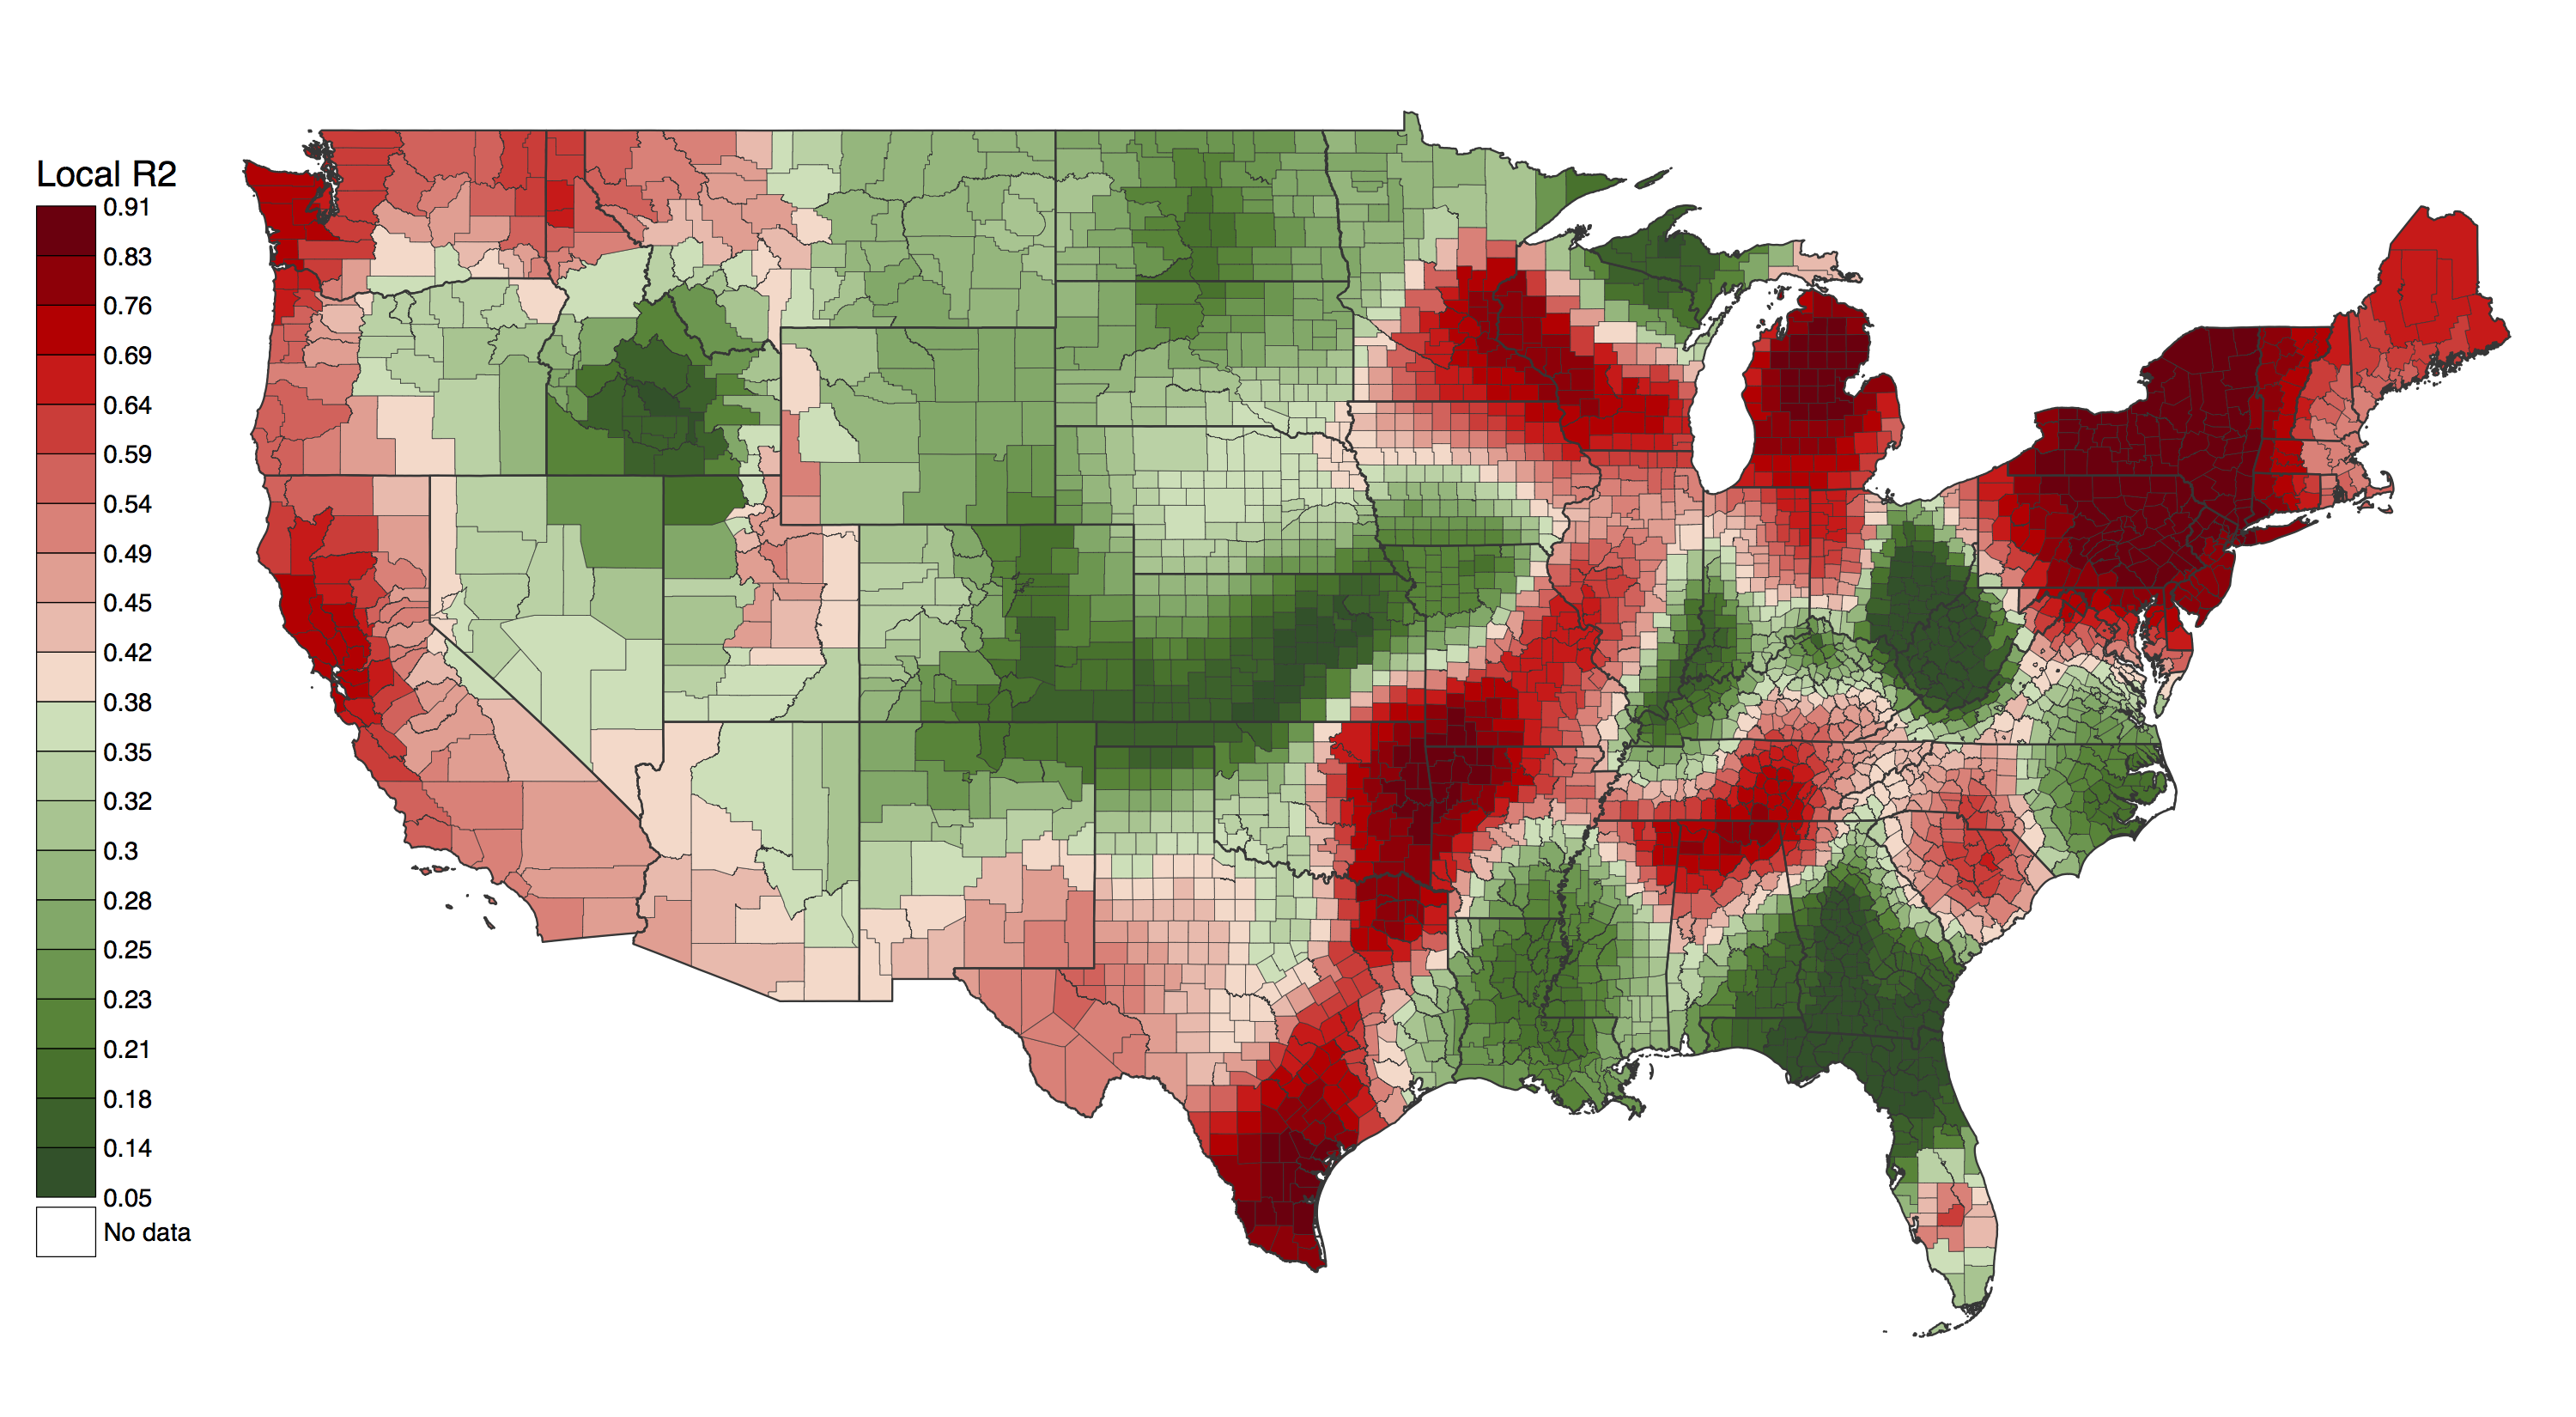
\includegraphics[width=0.5\textwidth,height=0.4\textheight]{figures/gwr_allbest_LocalR2}\\

}




\sframe{Multi-level Regression}{

% method of multi-level

%\begin{eqnarray}
%x_{i,s,c,t} &=& \beta_s + \varepsilon_{i,s,c,t} \\
%x_{i,s,c,t} &=& \beta_c + \varepsilon_{i,s,c,t} \\
%x_{i,s,c,t} &=& \beta_i + \varepsilon_{i,s,c,t}\\
%\end{eqnarray}

Fixed effect regression at the level of the state : multi-level modeling to capture spatial effect of administrative boundaries

\begin{equation}
\label{eq:reg}
log(x_{i}) = \beta_0 + X_{i}\beta_1 + \beta_{s(i)} + \varepsilon_{i},
\end{equation}

\medskip

\begin{itemize}
\item Clustering of standard error at the state level motivated by the strong spatial autocorrelation: capture county-level variation controlling for State fixed effect
\item Regressing the log of price on a state fixed-effect explains 74\% of the variance
\item influence of taxes: regressing the log of oil price on the level of state tax gives a R-squared of 0.33\%
\end{itemize}

}

\sframe{Multi-level Regression : results}{



\begin{table}[htbp]
\vspace{-0.1cm}
\begin{center}
\footnotesize
{
%\caption{\footnotesize{\textsc{Regressions at the county level}}}

\begin{tabular}{lccccc}
 %\toprule
 %\hline


  & (1) & (2) & (3) & (4) & (5) \\ 
%\cmidrule(r){2-6}
Density      &               &       0.016***&       0.016***&       0.016***&       0.015***\\
                    &               &     (0.002)   &     (0.001)   &     (0.001)   &     (0.001)   \\
Population (log)             &               &      -0.007***&      -0.040***&      -0.041***&      -0.039***\\                    &               &     (0.001)   &     (0.011)   &     (0.011)   &     (0.010)   \\
Total Income (log)            &               &               &       0.031***&       0.031***&       0.027***\\
                    &               &               &     (0.010)   &     (0.010)   &     (0.009)   \\
Unemployment        &               &               &       0.001   &       0.000   &       0.000   \\
                    &               &               &     (0.001)   &     (0.001)   &     (0.001)   \\
Poverty   &               &               &      -0.028** &      -0.030***&      -0.029** \\
                    &               &               &     (0.011)   &     (0.011)   &     (0.011)   \\
Percentage Black    &               &               &               &       0.000***&      -0.000   \\
                    &               &               &               &     (0.000)   &     (0.000)   \\
Vote GOP      &               &               &               &               &      -0.072***\\
                    &               &               &               &               &     (0.015)   \\ \cr 
%\cmidrule{2-6}
R-squared           &       0.743   &       0.767   &       0.774   &       0.776   &       0.781   \\
N                   &        3,066   &        3,011   &        3,011   &        3,011   &        3,011   \\
%\cr
%\hline
%\bottomrule
\end{tabular}
}
\end{center}
\end{table}


}



\sframe{Multi-level Regression : summary}{

\begin{itemize}
\item Strong influence of state-level tax
\medskip
\item Dense urban counties have higher fuel price, but price decreases with population 
\medskip
\item Fuel price increases with total income, decreases with poverty
\medskip
\item It decreases with the extent to which a county has voted for a Republican candidate: suggests a circular link
\medskip
\item Overall, local socio-economic features have explanatory power when removing State fixed effect
\end{itemize}


}







%%%%%%%%%%%%%%%%%
\section{Discussion}
%%%%%%%%%%%%%%%%%


\sframe{Implications}{

\justify

\textbf{Methodological}

\medskip

$\rightarrow$ Complementarity of Spatial analysis and econometrics methods : towards integrated approaches to territorial systems

\bigskip

\textbf{Practical}

\medskip

$\rightarrow$ Possible design of territory-targeted car-regulation policies, allowing both sustainability and territorial equity



}





\sframe{Possible Developments}{

\justify


$\rightarrow$ Microscopic data analysis (requires precise geocoding)

\bigskip

$\rightarrow$ Longer time series (collection in progress) and time-series modeling

\medskip

$\rightarrow$ Parametrization of a large-scale ABM of the spatialized fuel market : investigation of  adaptive policies effects at the local and global level

\medskip

$\rightarrow$ Scales and ontologies to study relations between network and territories




}



\sframe{Conclusion}{

$\rightarrow$ A novel insight into spatio-temporal dynamics of fuel price and their determinants thanks to big data harvesting

\medskip

$\rightarrow$ Complementary approaches and conclusions through GWR and multi-level modeling


\bigskip
\bigskip
\bigskip


\footnotesize{ - All code available at \texttt{https://github.com/JusteRaimbault/EnergyPrice}

\medskip

 - Raw dataset available upon request

\medskip

 - Paper preprint available at \texttt{http://arxiv.org/abs/1706.07467}
}

}






%%%%%%%%%%%%%%%%%%%%%
\begin{frame}[allowframebreaks]
\frametitle{References}
\bibliographystyle{apalike}
\bibliography{biblio}
\end{frame}
%%%%%%%%%%%%%%%%%%%%%%%%%%%%





%%%%%%
\sframe{Spatial Heterogeneity}{

Spatial Autocorrelation as an index of spatial variability, for link $i$

\begin{equation}
\rho_i = \frac{1}{K}\cdot \sum_{i\neq j}{w_{ij}\cdot (c_i - \bar{c})(c_j - \bar{c})}
\end{equation}

with spatial weights  $w_{ij} = \exp{\left(\frac{-d_{ij}}{d_0}\right)}$

}



%%%%%%
\sframe{GWR Residuals}{

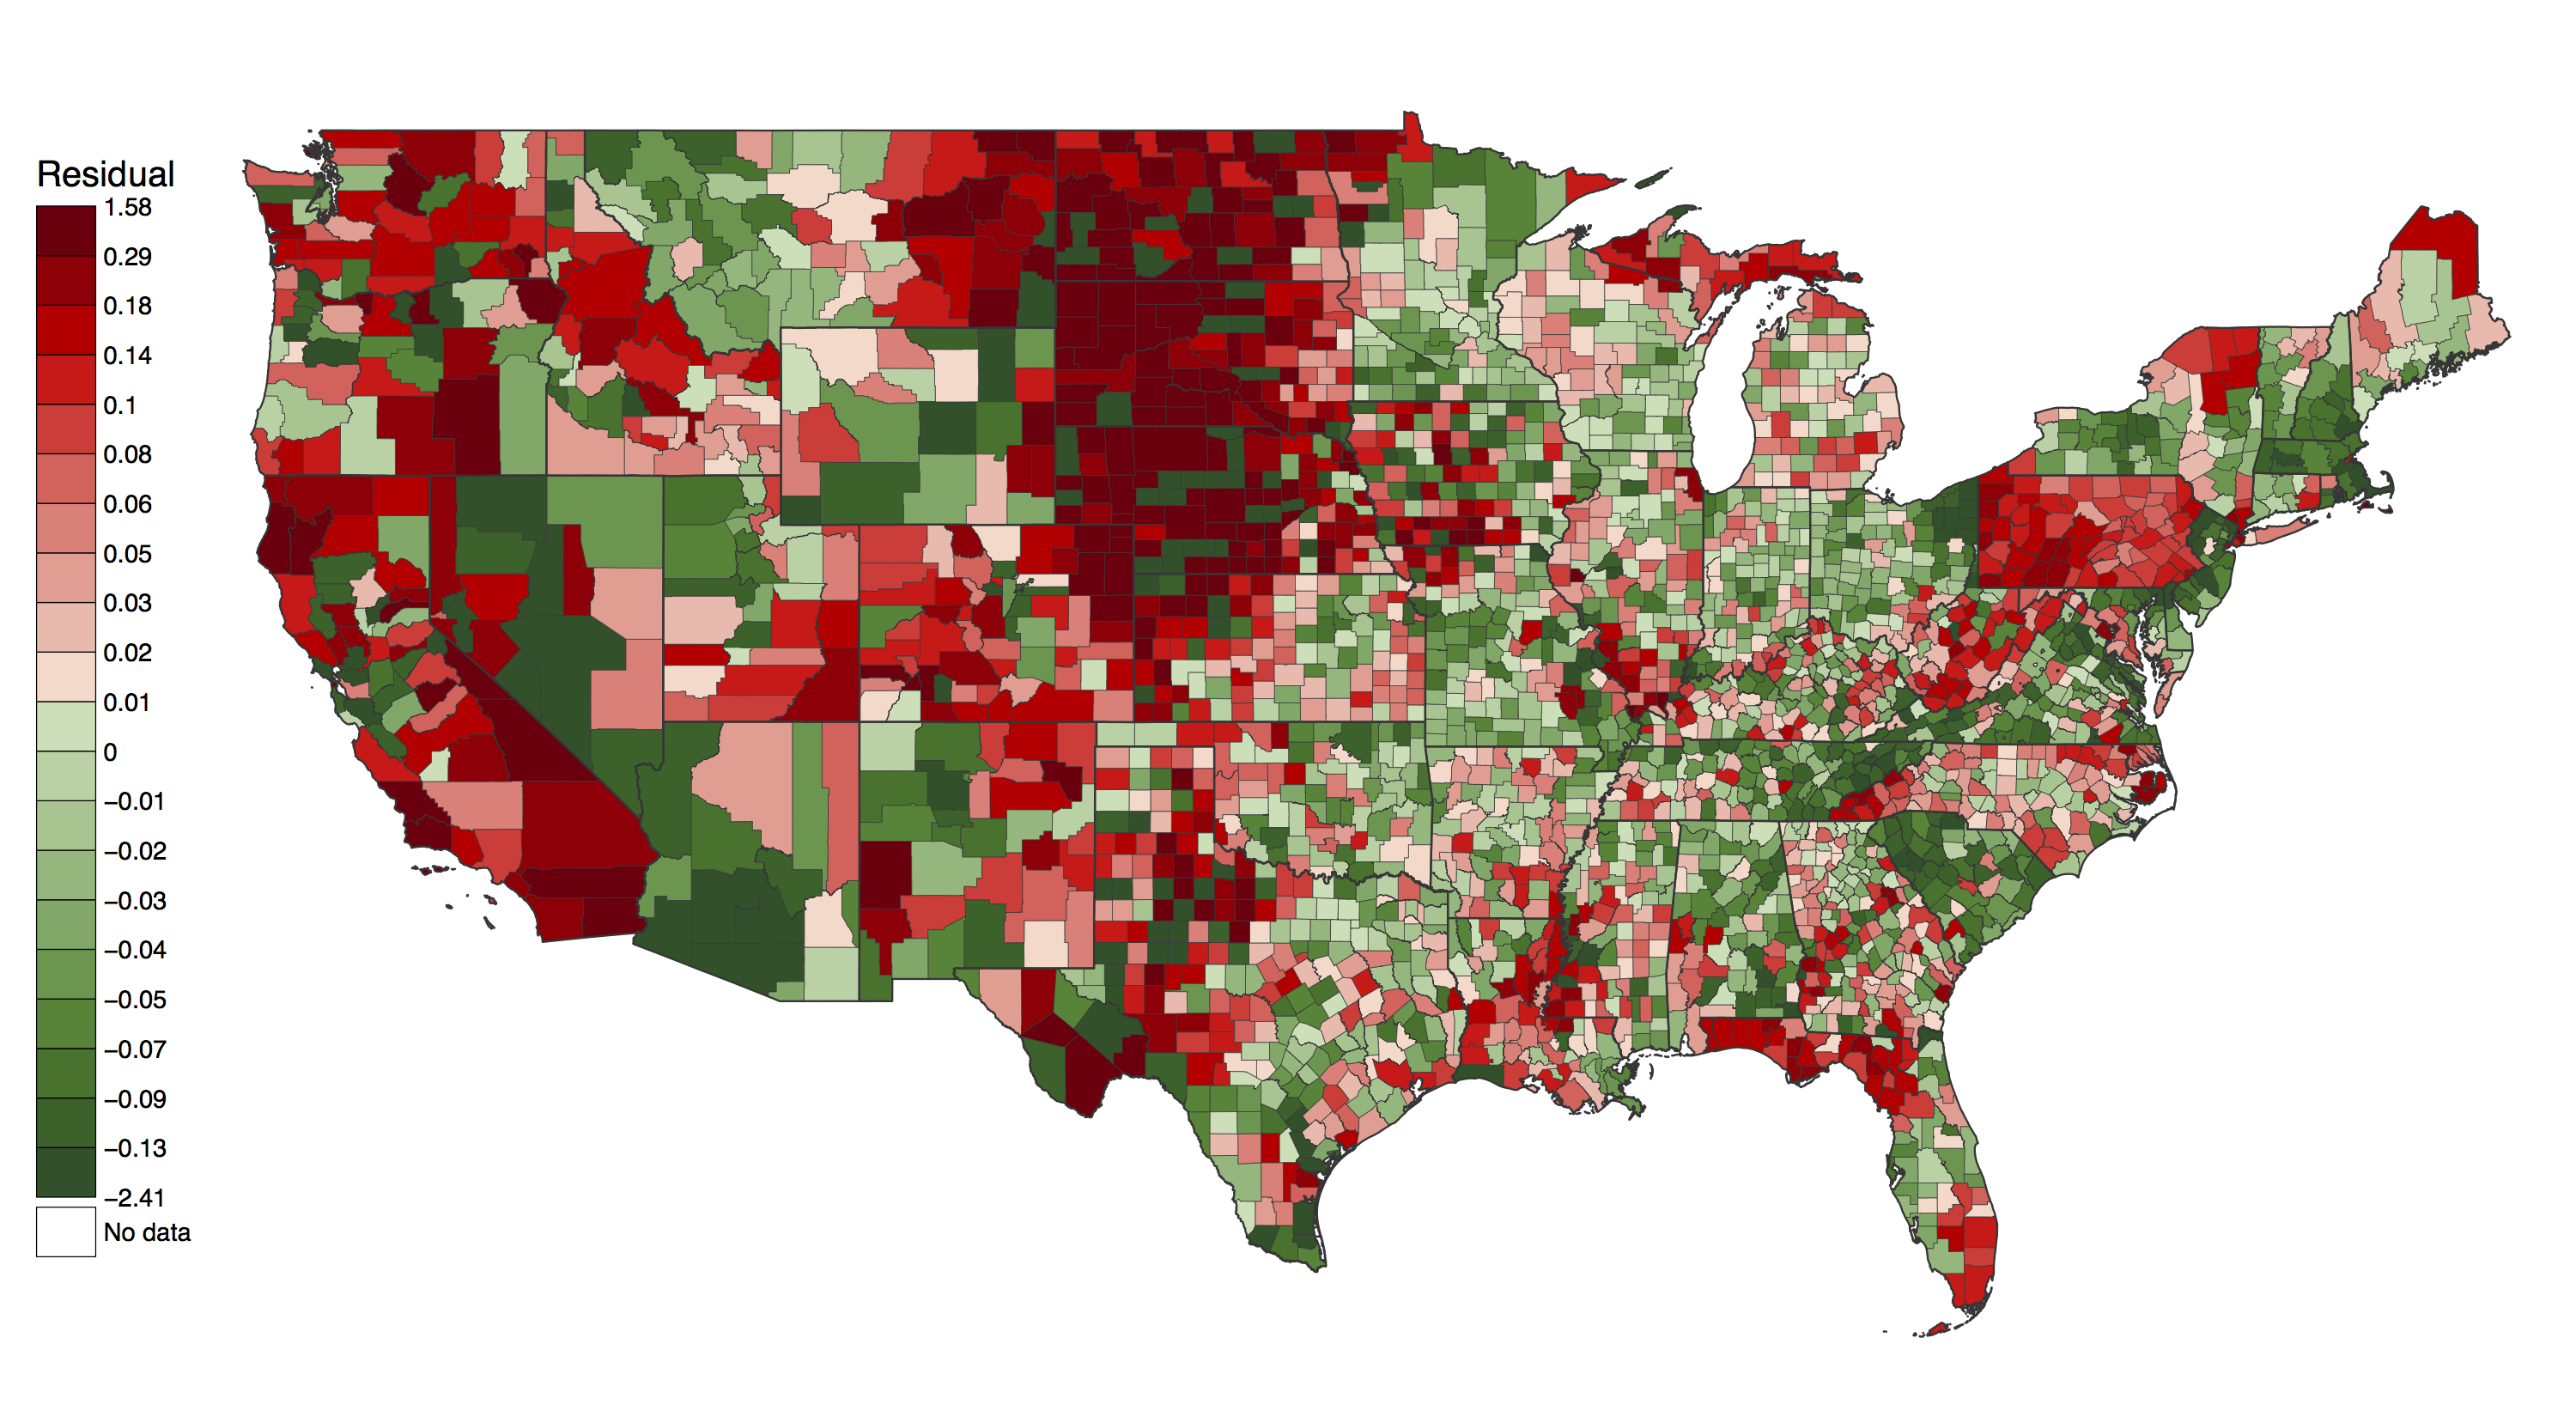
\includegraphics[width=0.8\textwidth]{figures/gwr_allbest_residual}

}






\end{document}







